%%%%%%%%%%%%%%%%%%%%%%%%%%%%%%%%%%%%%%
% This is the name of the style file.
%%%%%%%%%%%%%%%%%%%%%%%%%%%%%%%%%%%%%%
%
% phd  -> for a PhD dissertation
% ms   -> for an MS thesis
% If both phd and ms are used then phd will overide.  If none are used,
% then ms will be active by default.
%
% cpyr -> generate a copyright page
% lof  -> generate List of Figures
% lot  -> generate List of Tables
\documentclass[ms,cpyr,lof,lot]{uathesis}
%\documentclass[ms]{uathesis}
%
%%%%%%%%%%%%%%%%%%%%%%%%%%%%%%%%
% List of any packages you use.
%%%%%%%%%%%%%%%%%%%%%%%%%%%%%%%%
%
\usepackage{amsmath}
\usepackage{amssymb}
\usepackage{graphicx}

\usepackage{listings}
\usepackage{color}
\usepackage{setspace}
\usepackage{subcaption}
\usepackage[table]{xcolor}
\usepackage{textcomp}

%
%%%%%%%%%%%%%%%%%%%%%%%%%%%%%%%%%%
% List of definitions you define.
%%%%%%%%%%%%%%%%%%%%%%%%%%%%%%%%%%
%
\def\ds{\displaystyle}
\def\E{\epsilon}
\def\eps{\varepsilon}
\definecolor{lightgray}{gray}{0.9}


\title{A simple Coarse-grained model of a Carbon Nanotube Forest interacting with a rigid substrate}
\author{Andrew Robert Marmaduke}
\conferraldate{May}{2015}

%The following commands specify the names and titles of people that
%will appear on the signature page.
%
%These four will always be needed.
\advisor{Dr. Dimitry Golovaty}
\chair{Dr. Timothy Norfolk}
\collegedean{Dr. Chand Midha}
\gradschdean{Dr. Rex D. Ramsier}
%
%For a PhD dissertation, specify a coadvisor and three committee
%members, or four committee members only.  For an MS thesis use either
%one coadvisor or one faculty reader, not both.
%
%Typical commands for a PhD dissertation (uncomment only 4).
%\coadvisor{Dr. J Patrick Wilber}
%\committee{Name of 1st Comm Member}
%\committee{Name of 2nd Comm Member}
%\committee{Name of 3rd Comm Member}
%\committee{Name of 4th Comm Member}
%
%Typical commands for an MS thesis (uncomment only 1).
\coadvisor{Dr. J Patrick Wilber}
\facreader{Dr. Gerald Young}
%\facreader{Name of Fac Reader}

\begin{document}
\maketitle
\chapter{INTRODUCTION} \label{chap:one}

\section{Graphene and carbon nanotubes}

	Graphene is a configuration of covalently bonded carbon atoms arranged in a two-dimensional hexagonal lattice. It is known to be a structural component to graphite, carbon nanotubes, and other materials. However, the existence of stable graphene sheets was only speculative, until they were isolated experimentally in 2004 \cite{Novoselov2004}. Graphene has many potential applications, primarily because of the high Young's modulus, room temperature electron mobility, thermal conductivity, optical absorption, gas impermeability, etc \cite{Novoselov2012}. Recently developed novel transistors \cite{Lin2010} and composite materials for solar cells \cite{Wang2013} emphasize the future promise of graphene. Mass production of an acceptable quality of graphene is, however, still in its infancy, and with it so are industrial applications \cite{Novoselov2012}.
	
	\begin{figure}
		\begin{center}
			\def\svgwidth{.75\columnwidth}
			\input{./fig/ch1/chirality.eps_tex}
		\end{center}		
		\caption{A graphene sheet with possible choices of a chiral vector $\mbox{C}_{\textbf{v}}$.
		\label{fig:GrapheneCat}}
	\end{figure}

	Carbon nanotubes were first identified in 1950's although they were brought to the attention of the wider scientific community in 1991 \cite{Iijima1991}. A carbon nanotube (CNT) can conceptually be thought of as an appropriately rolled graphene lattice (see Fig.~\ref{fig:GrapheneCat}). CNTs are categorized by their chirality and the number of encasing shells. A CNT is called a single-walled carbon nanotube (SWCNT) if there is only one cylindrical structure with no additional interior or exterior CNTs, a double-walled carbon nanotube (DWCNT) if there is exactly two concentric CNTs, or a multi-walled carbon nanotube (MWCNT) if there are more than two. Chirality of a CNT is categorized by a vector on a graphene sheet. The basis for this vector is shown on Fig.~\ref{fig:GrapheneCat}, $a_1$ and $a_2$, which forces head and tail points to lie on vertices of a hexagon. A CNT is then formed by rolling the graphene sheet along the vector, $\mbox{C}_{\textbf{v}}$, until the head and tail points meet. In this way $\mbox{C}_{\textbf{v}}$ determines the circumference of the CNT and an orthogonal vector T is the tube axis. The tail is usually taken as a reference or origin point, and then chirality is determined by the position of the head. 
A CNT is called armchair if along the tube axis the hexagon structure repeats uniformly (see Fig.~\ref{subfig:Armchair}), zigzag if the hexagon structure alternates (see Fig.~\ref{subfig:Zigzag}), and chiral otherwise.
	
	Like graphene, CNTs have many desirable properties. In particular, depending on the structure of a CNT, a tube behaves either as a semiconductor or a metal, has an effective Young's modulus comparable to graphene, and has high thermal conductivity \cite{Dresselhaus2004}. Both graphene and CNTs have strong molecular bonds between carbon atoms which makes them highly resistant under tension, but each bond allows small deformations which can lead to a large curvature of two-dimensional nanostructures. Moreover, under heavy strain CNTs can relax via Stone-Walls diatomic interchange creating sharper bends and deformation \cite{Yakobson1998}. CNTs are already being used in industrial applications from lithium ion batteries to composite bicycle frames \cite{De2013} with future applications being researched.
	
	\begin{figure*}[t!]
		\centering
		\begin{subfigure}[t]{.5\textwidth}
			\centering
			\input{./fig/ch1/armchair.eps_tex}
			\caption{\label{subfig:Armchair}}
		\end{subfigure}%
		~
		\begin{subfigure}[t]{.5\textwidth}
			\centering
			\input{./fig/ch1/zigzag.eps_tex}
			\caption{\label{subfig:Zigzag}}
		\end{subfigure}		
		\caption{Chirality of a CNT can be depicted by how often a hexagonal pattern repeats along a consistent axis. A CNT is (a) armchair if every hexagon is the same, (b) zigzag if the pattern alternates every two hexagons, and chiral otherwise.\label{fig:Chirality}}	
	\end{figure*}
	
\section{Carbon-nanotubes-based materials}

By Carbon-nanotubes-based materials, we mean materials that consist entirely (except for possibly a substrate) of CNTs and no additional materials like polymers.	
The macroscopic properties of CNTs-based materials are dependent on several factors: purity, porosity, and alignment being a few.
A CNT forest, turf, or array is a structure consisting of several CNTs grown from a substrate.
One method for producing CNT forests is chemical vapor deposition.
CVD has been used in nano-electronic fabrication and is not a new technology.
When considered for CNTs it allows for targeted growth on a substrate which is a desirable property for designing and making electronic applications.
CVD is thought to have the best potential for commercial success \cite{Nessim2010}.
A simplified description of CVD is of a furnace that energizes a gas and substrate (usually with some catalyst) to cause a chemical bonding of gas particles with the substrate.
In the case of CNTs the gas consists of hydrocarbons and several different catalysts have been tried and tested.
However, the exact mechanism of CNT growth in a CVD process is complicated by factors such as chemical processes depending on the catalyst, ballistics involving the CNT length \cite{Louchev2003}, and temperature of the CVD.
The quality of the CNT forest can vary greatly and has been considered more of an art than a science \cite{Nessim2010}.  
	
Vertically aligned carbon nanotubes (VACNTs) are used in several different applications.
The electrical and thermal conductivity of CNT materials are highly dependent on the alignment bias of the material.
Likewise adhesive and optical properties of VACNTs are very dynamic and depend on structure, uniformity, purity and other factors.
VACNTs can be used as hydrophobic materials \cite{Lau2003}, dry adhesives \cite{Chen2012}, hologram generators \cite{Montelongo2013}, and nano-workbenches \cite{Gjerde2006}.
VACNTs have an adhesive property and simultaneously have low static friction which plays a critical role in the hydrophobic, and workbench applications.
Xu et al. demonstrate a crowding effect of CNT arrays that allows for control of CNT alignment \cite{Xu2012}.
The structure of a forest can also be used to spin yarns.
A super-aligned array of CNTs can be spun into a yarn of lengths up to centimeters or more \cite{Jiang2002}.
	
A film of CNTs, with no necessary alignment bias or connection to a substrate, is called buckypaper.
Buckypaper is assembled in several ways, including layer-by-layer deposition of functionalized MWCNTs \cite{Lee2008} and ``domino pushing'' of a CNT array.
The relative properties of buckypaper are dependent on the assembly method.
Wang et al. describe the ``domnio pushing'' method as pressing a micropore membrane onto a CNT array.
The membrane is pushed by a cylinder with constant pressure from one end to the other of the CNT array causing individual CNTs to collapse in a ``domino'' fashion.
The CNTs then stick to the membrane and can be peeled off a silicon substrate and then treated and peeled off the membrane \cite{Wang2008}.
A buckypaper assembled with ``domino pushing'' of a highly aligned CNT array will also have an alignment bias, whereas a layer-by-layer deposition will be randomly distributed.

CNTs are often used as a reinforcing agent in composite materials, for example as dispersed CNTs in an epoxy deposit to improve mechanical strength.
A common method of constructing composite materials is through solvents.
In a process involving solvents, CNTs are dispersed with a polymer material and then the solvent is carefully evaporated.
Uniform dispersion of CNTs is a primary concern for mechanical reinforcement, where ideally the stress applied to a material would be augmented by the strength of the reinforcing tubes \cite{Coleman2006}.
There are several composite and reinforcement processes that have been explored and that have varying effectiveness to create an improved composite material.
Spitalsky et al. review several processes and discuss properties of corresponding composites \cite{Spitalsky2010}.

\begin{figure*}[t!]
		\centering
		\begin{subfigure}[t]{.33\textwidth}
			\centering
			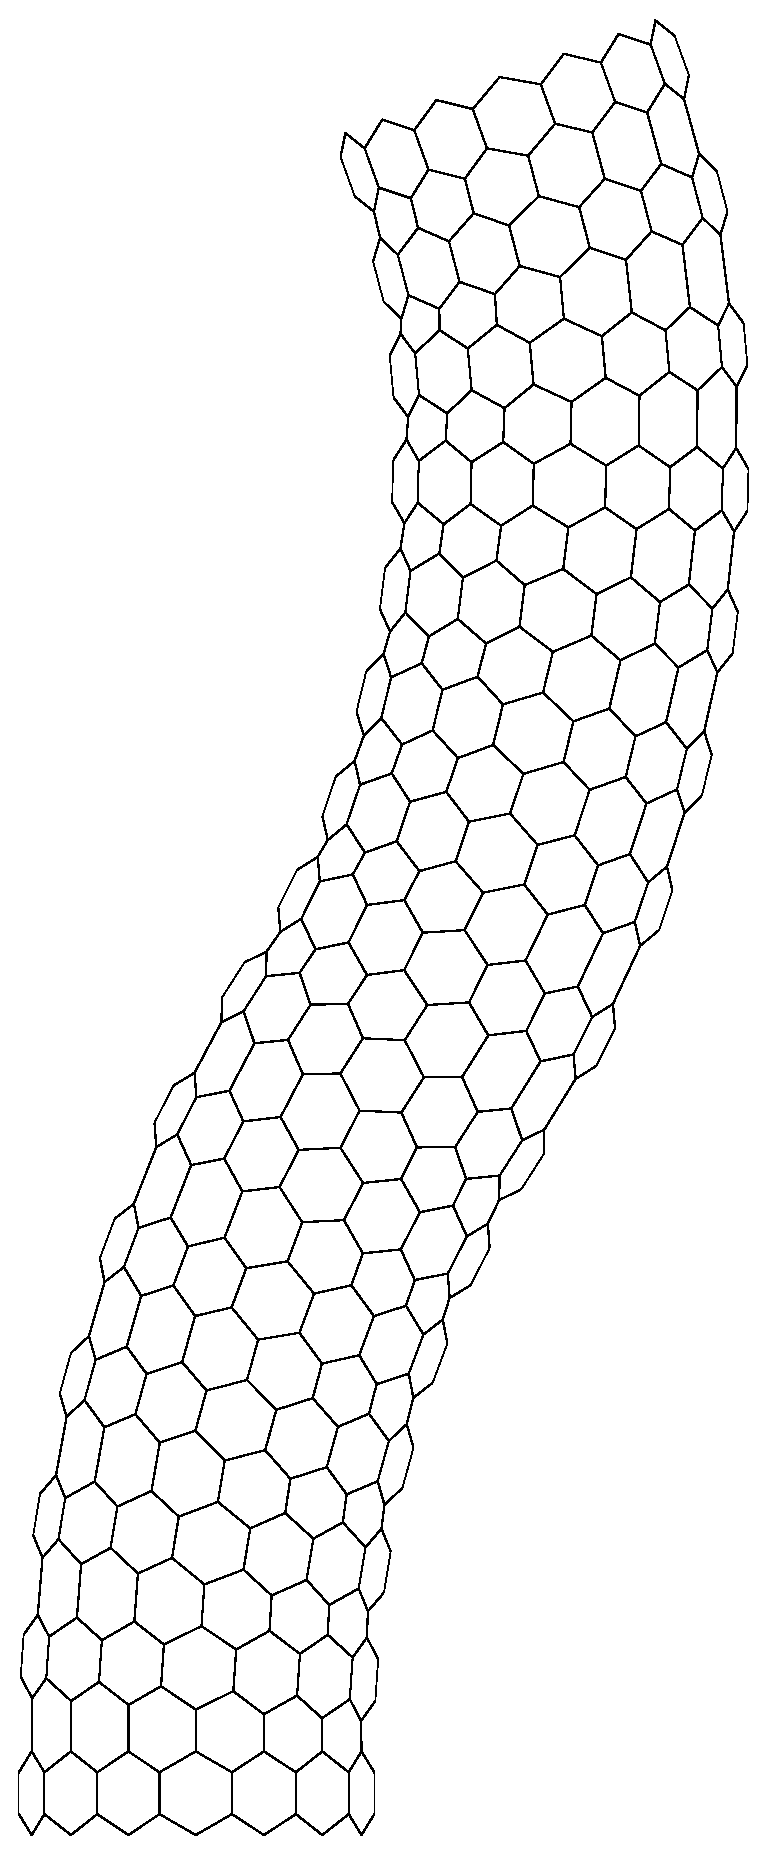
\includegraphics{./fig/ch1/Nanotube.eps}
			\caption{\label{subfig:Nanotube}}
		\end{subfigure}%
		~
		\begin{subfigure}[t]{.33\textwidth}
			\centering
			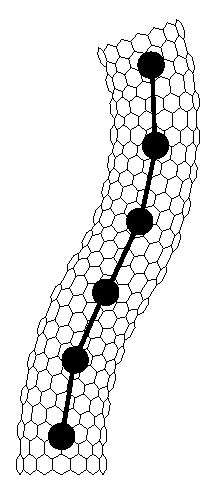
\includegraphics{./fig/ch1/NanotubeParticle.eps}
			\caption{\label{subfig:NanotubeParticle}}
		\end{subfigure}%
		~		
		\begin{subfigure}[t]{.33\textwidth}
			\centering
			\includegraphics{./fig/ch1/NanotubeCylinder.eps}
			\caption{\label{subfig:NanotubeCylinder}}
		\end{subfigure}
		\caption{There are several ways to model a CNT with a coarse-grained approach. (a) A CNT under torsional strain can be depicted as (b) a particle bead-spring model of a CNT or (c) a sequence of cylinders model of a CNT. \label{fig:CoarseGrain}}	
	\end{figure*}

\section{Models of buckypaper and fiber materials}

	CNTs in buckypaper can be modeled as individual fibers due to their aspect ratio and flexibility. Indeed, any material consisting of a large volume of CNTs can be thought of as a fiber material. Fiber materials or films are modeled at various length scales. Molecular dynamics takes a small collection of particles and describes their motion with some governing dynamical system for a short period of time. Full atomistic simulations of fiber structures are generally speaking impractical for a large number of atoms or long time scales. For example, investigation of the heat conductance of a single CNT is a practical consideration for molecular dynamics simulations \cite{Maruyama2003}. In order to investigate longer length and time scales coarse-grained approaches are used. The exact time and length scales that are appropriate for different computational techniques are difficult to quantify. With consistently improving hardware and better algorithms and techniques to handle error propagation the line is steadily shifting. However, qualitatively, molecular dynamics approaches will always be focused on a shorter time scale and smaller systems than coarse-grained approaches which in turn are effective at smaller scales than finite element methods \cite{Muller2002}.
	
	Coarse-grained techniques applied to fiber materials model a collection of atoms as a single particle, encapsulating the motion of an entire fiber as a chain of linked particles, instead of a molecular structure of bonded atoms. The focus of coarse-grained simulations is on the mesoscopic scale, somewhere between 1 nanometer and 1 micrometer.  There are many variations to coarse-grained fibers: the fiber can be thought of as a single rod with an attached particle (or a ``lollipop'') \cite{Buehler2006}, a collection of bead-spring links \cite{Li2012} (see Fig.~\ref{subfig:NanotubeParticle}), or a sequence of cylinders \cite{Volkov2008} (see Fig.~\ref{subfig:NanotubeCylinder}).
	
After a model and set of governing equations is developed, the next concern is constructing initial data.
When dealing with a fiber material or mesh with hundreds of fibers, manual generation of initial data is impractical.
Thus appropriate and careful construction of the initial configuration is a concern.
Preventing fibers from penetrating each other and obtaining a desired volume fraction are two of the issues involved in constructing self-consistent initial data.
Dalmas et al. modeled fibers as several splines \cite{Dalmas2006}, however there was no inner volume to each fiber due to an effective zero radius of the fibers which made it difficult to construct a mesh of a desired volume fraction.
Altendorf and Jeulin address this issue with random walks of spheres that can shrink to ``squeeze'' through holes allowing for low porosity \cite{Altendorf2011}.
Cranford et al. construct an array of fibers independently of the mesh and then sediment each array onto a surface \cite{Cranford2010}.

\section{Models of fiber adhesion}

Van der Waals interaction is a combination of several interatomic forces (both repulsive and attractive).
Van der Waals interaction has been considered as a predominant force in adhesive materials (e.g. dry adhesion of Gecko setae \cite{Autumn2002}), and has been used to investigate properties of mesoscopic fibers (e.g. spider silk fibrils \cite{Cranford2013}).
The models we consider here are those that consider van der Waals interaction as a critical mechanism for adhesion of a fiber or fiber material.
A model of fiber adhesion incorporates fibers and possibly other structures like substrates with some adhesive force.
Although fiber only adhesion can and has been considered \cite{Li2011}, we focus on adhesion involving substrates. 
	
	Fu and Zhang utilized an exact continuum model to investigate peeling of a fiber off a substrate \cite{fu2011}. Majidi introduced a continuum model for fiber adhesion with an upper substrate, in particular focusing on the adhered length of a fiber as a function of the applied normal and shear force \cite{Majidi2009}. Majidi's model was later expanded by He et al. to include a coupling effect between shear and normal force \cite{He2012}, and then later to include an axial strain \cite{He2013}. 
	
	To model several interacting fibers, finite element methods have been used \cite{Radhakrishnan2013}. Hu et al. take a multiscale approach adapting coarse-grained molecular dynamics and finite element method to model an array of fibers between two substrates \cite{Hu2010}. Yang et al. investigate a similar problem with only coarse-grained fibers \cite{Yang2012}.
	
	Models of fibers with an adhesive mechanism follow several patterns in the governing energies or forces. Both Hu et al., and Yang et al. include at least a bending energy, axial energy, and short-range potential. Yang et al. stochastically add springs between neighboring fibers to reinforce the several vertically aligned fibers close to the bottom substrate. If there is an axial energy between particles in a coarse-grained fiber it is usually treated as an extensible spring, however inextensible equivalents also exist. The bending of a fiber is usually determined by the interior angle of contiguous particles along the fiber. Finally, the short-range potential models the van der Waals interaction inter-fiber or between fiber and potentially other objects like substrates. 

	We take a similar approach using a simple coarse-grained model with an axial, bending, and short-range weak interaction energies. We also include two substrates, one of which can be rigidly translated by an applied load. The vdW interaction between the fiber and the substrates is explored as a type of adhesion.
	
\section{Summary}

We consider a system consisting of one or more fibers constrained between two parallel substrates where one substrate is stationary, while the other substrate can move. 
The fibers are assumed to be physically attached to the stationary substrate. 
They can be stretched or bent and are subject to non-local self-interactions as well as van der Waals interactions with other fibers and both substrates. 

In Chapter 2, we formulate a coarse-grained model of the fibers/substrates system in which the fibers are replaced by chains of discrete particles connected by extensional and torsional springs and implement this model numerically. 
We assume that dynamics of the system is dominated by dissipative effects and thus can be described in terms of a gradient flow. 

In Chapters 3 and 4, we perform a number of numerical experiments to study the adhesive properties of the fibers. 
First, in Section 3.1, we discard the movable substrate and consider a fiber initially attached orthogonally to the stationary substrate. 
We then determine an equilibrium configuration that results from relaxing the fiber over time. 
We observe that the fiber can either remain free-stranding or adhere to the substrate, e.g., if the torsional springs are sufficiently weak. 
Note that, as in all of our simulations, the equilibrium configuration corresponds to a local minimizer of the energy.

In the next set of experiments in Section 3.2, we reintroduce into the system the rigid movable substrate. 
This (top) substrate can undergo translational motion while remaining parallel to the stationary (bottom) substrate to which the fiber is attached. 
The top substrate is assumed to interact with the fiber via van der Waals forces. Loads of various magnitudes are applied at different angles to the top substrate causing the fiber to deform and adhere to one or both substrates. 
We analyze the set of resulting equilibrium configurations and discuss the dependence of these configurations on material parameters of the system.

The compression experiment is followed by the study of the fiber detachment in Section 3.3, where the sign of the load acting on the top substrate is reversed. 
We investigate dynamics of detachment and identify possible detachment mechanisms. 
Finally, in Chapter~\ref{chap:four}, we present some preliminary results for a two substrate system with multiple fibers.
\chapter{Model} \label{chap:two}

% Parameter Table
\begin{table}
	\rowcolors{1}{}{lightgray}
	\centering
	\caption{Model parameters. \label{table:parameters}}
	\begin{tabular}{c p{.25in} p{4.5in}}
		$m$ & & Number of fibers \\
		$n_j$ & & Number of particles on the $j$th fiber, $1 \leq j \leq m$ \\
		$n_+$ & & Number of particles on the top substrate \\
		$n_-$ & & Number of particles on the bottom substrate \\
		$\delta_j$ & & Attachment point for the $j$th fiber on the bottom substrate, $1 \leq j \leq m$ \\
		$\ell$ & & Equilibrium distance for extensible springs \\
		$\ell_+$ & & Spacing between particles on the top substrate \\
		$\ell_-$ & & Spacing between particles on the bottom substrate \\
		$\beta$ & & Strength of torsional springs \\
		$\gamma$ & & Spring constant for extensible springs \\
		$\varepsilon$ & & Strength of vdW force between particles of fibers \\
		$\varepsilon_+$ & & Strength of vdW force between a particle on a fiber and a particle on the top substrate \\
		$\varepsilon_-$ & & Strength of vdW force between a particle on a fiber and a particle on the bottom substrate \\
		$\sigma$ & & Equilibrium distance between two particles for vdW \\
		$(\mu,\lambda)$ & & Load applied to the moving substrate \\
		$(x^{(+)}_0,y^{(+)}_0)$ & & Initial position for first particle on the top substrate \\
		$(x^{(-)}_0,y^{(-)}_0)$ & & Initial position for first particle on the bottom substrate
	\end{tabular}
\end{table}
	
	\begin{figure}
		\begin{center}
			\input{./fig/ch2/geometry.eps_tex}
		\end{center}		
		\caption{Geometry of a fiber pinned between the top and bottom substrates.
		\label{fig:Geometry}}
	\end{figure}		
	
\section{Geometry}

   We consider a collection of particles linked into a chain that we call a fiber. Each fiber is connected to a stationary horizontal (bottom) substrate at some fixed position. We also consider a (top) substrate that is always parallel to the bottom substrate and that only translates. There are two artificial particles associated with each fiber, one at the connection (or attachment) point with the bottom substrate and an additional particle placed at any point on a half circle below the bottom substrate of radius one. We call the particle at the attachment point the attachment particle, and the other particle below it the floating particle (see Figure~\ref{fig:Geometry}). The system consists of $m$ fibers, with $n_j$ particles for the $j$th fiber, a top substrate with $n_+$ particles, and a bottom substrate with $n_-$ particles.
	
We denote the position vector of the $i$th particle on the $j$th fiber by
\begin{equation}
	\textbf{r}_i^{(j)} = (x_i^{(j)},y_i^{(j)})
\end{equation}
where $1 \leq j \leq m$ and $1 \leq i \leq n_j$. We also define the following vectors for convenience,
\begin{equation}
	\Delta \textbf{r}_i^{(j)} = \textbf{r}_i^{(j)} - \textbf{r}_{i-1}^{(j)}.
\end{equation}
The two artificial particles are denoted as follows,
\begin{equation}
	\textbf{r}_0^{(j)} = (x_0^{(j)},y_0^{(j)}) = (\delta_j,0)
\end{equation}
for the attachment particle and
\begin{equation}
	\textbf{r}_{-1}^{(j)} = (x_{-1}^{(j)},y_{-1}^{(j)}).
\end{equation}
for the floating particle.

	The chain of particles is a discrete analog to a CNT (see Figure~\ref{subfig:NanotubeParticle}). Indeed, the vectors $\Delta \textbf{r}_i^{(j)}$ conceptually represent the interparticle bonds in this geometry. However, this approach is sufficiently generic to describe other fiber structures and we do not limit our discussion to this motivation.
	
	The bottom substrate as described before is attached to every fiber at the attachment particle. We define two position vectors,
\begin{eqnarray}
	\textbf{r}_0^{(+)} = (x_0^{(+)},y_0^{(+)}) & \\
	\textbf{r}_i^{(+)} = (x_0^{(+)} + i\ell_+,y_0^{(+)}), & 0 < i < n_+
\end{eqnarray}
for the top substrate and,
\begin{eqnarray}
	\textbf{r}_0^{(-)} = (x_0^{(-)},y_0^{(-)}) & \\
	\textbf{r}_i^{(+)} = (x_0^{(+)} + i\ell_-,y_0^{(+)}), & 0 < i < n_-
\end{eqnarray} 
for the bottom substrate. Since both substrates are rigid, the bottom substrate is stationary, and the top substrate is only allowed to translate, the positions of all particles on each substrate can be respectively specified by identifying the position of a single particle. Both particles are decided as initial conditions together with the initial positions of every particle on each fiber. The rest of the particles on either substrate are defined by a parameter for the total number of particles, and an interval spacing, $\ell_+$ and $\ell_-$.

\section{Energy}

	We want a fiber to be in equilibrium when all particles are collinear and each particle is a fixed distance $\ell$ away from its neighbors. In order to enforce this equilibrium configuration we incorporate two types of springs into the model: an extensible spring and a torsional spring.

\subsection{Extensible spring}

	The extensible spring is described by the standard Hooke's law with spring constant $\gamma$ and is meant to keep any two adjacent particles on a fiber a fixed distance $\ell$ apart. The energy for all extensible springs in the system is then
\begin{equation}
	E_e = \gamma \sum_{j=1}^m \sum_{i=1}^{n_j} \left[ \left( \|\Delta \textbf{r}_i^{(j)} \| - \ell \right)^2 \right].
\end{equation}
Note that there is no spring between the floating particle and the attachment particle, but there is a spring between the attachment particle and the $\textbf{r}_0^{(j)}$ particle on the $j$th fiber. Both the attachment particle and the floating particle are introduced into the system to model the connection between the fiber and the bottom substrate. The spring between the attachment particle, $\textbf{r}_0^{(j)}$, and the particle, $\textbf{r}_1^{(j)}$, enforces attachment of the $j$th fiber.

	\begin{figure}
		\begin{center}
			\input{./fig/ch2/torsionenergy.eps_tex}
		\end{center}		
		\caption{Two vectors $\textbf{a}$ and $\textbf{b}$, representing links between three particles and a corresponding angle measured against the positive $x$-axis centered at each tail point. The bending energy will be minimized when the difference in angle is zero, or the particles are collinear.
		\label{fig:BendingEnergy}}
	\end{figure}	

\subsection{Torsional spring}

	The extensible springs alone are not sufficient to describe the kind of equilibrium we seek, so we introduce an energy penalty for bending, when the adjacent particles are not collinear (see Figure~\ref{fig:BendingEnergy}). We choose the expression,
\begin{equation}
	e_b = 2\beta \tan^2 \left( \frac{\Delta \theta}{2} \right),
\end{equation}
to represent the energy of a torsional spring at the junction between two bonds. Here $\beta$ is the strength of the spring. Notice this energy diverges as $\Delta \theta \to \pm180$\textdegree to guarantee that the bonds to do fold onto themselves. The geometry of the system is described in terms of particles, not angles, hence we rewrite the energy in terms of position vectors,
\begin{equation}
	E_b = 2\beta \sum_{j=1}^m \sum_{i=1}^{n_j} \left[ \frac{\|\Delta \textbf{r}_i^{(j)} \| \|\Delta \textbf{r}_{i-1}^{(j)} \| - \Delta \textbf{r}_i^{(j)} \cdot \Delta \textbf{r}_{i-1}^{(j)}}{\|\Delta \textbf{r}_i^{(j)} \| \|\Delta \textbf{r}_{i-1}^{(j)} \| + \Delta \textbf{r}_i^{(j)} \cdot \Delta \textbf{r}_{i-1}^{(j)}} \right].
\end{equation}

	This energy incorporates every contiguous set of three particles, including the two artificial particles. With the incorporation of the angle between the artificial particles and the particle, $\textbf{r}_0^{(j)}$, the optimal angle of the fiber with respect to the substrate can be tuned according to the placement of the floating particle. For example, if the angle between the artificial bond connecting the floating particle to the attachment particle, and the first bond connecting the attachment particle to particle $\textbf{r}_0^{(j)}$ is $90$\textdegree, then the entire fiber will want to be upright. If the equilibrium attachment angle is $45$\textdegree, then the entire fiber will want be slanted at $45$\textdegree,~etc. 

   The system of extensible and torsional springs is sufficient to model the equilibrium behavior of a system of isolated noninteracting fibers. However, we are still motivated by a nanoscale setting, namely that of CNTs. We introduce a particle-particle interaction to model the kinds of molecular forces we would expect on a nanoscale.

\subsection{van der Waals interactions}	

	\begin{figure*}[t!]
		\centering
		\begin{subfigure}[t]{.5\textwidth}
			\centering
			\includegraphics[scale=.5]{./fig/ch2/lj_e.eps}
			\caption{Lennard-Jones energy, well depth is $\varepsilon$, minimized at $\sigma$. \label{subfig:LJEnergy}}
		\end{subfigure}%
		~
		\begin{subfigure}[t]{.5\textwidth}
			\centering
			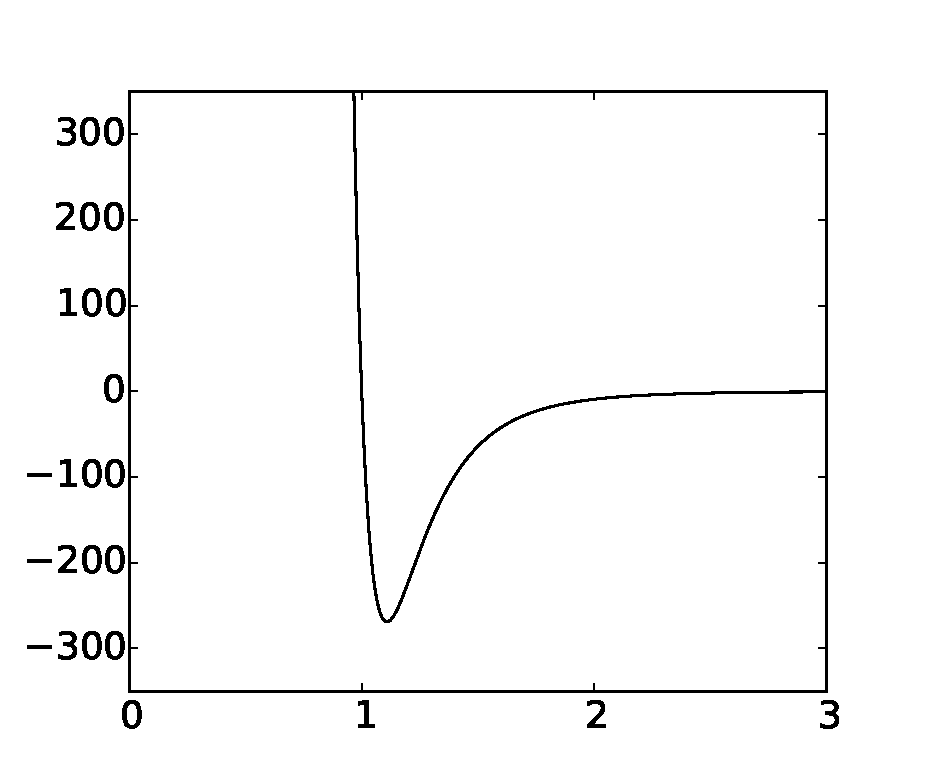
\includegraphics[scale=.5]{./fig/ch2/lj_f.eps}
			\caption{Lennard-Jones force. \label{subfig:LJForce}}
		\end{subfigure}		
		\caption{Lennard-Jones 12-6 potential and force with $\sigma = 1$ and $\varepsilon = 100$.\label{fig:LJ}}	
	\end{figure*}

   Van der Waals' (vdW) interaction are used to describe the sum of attractive and repulsive forces of atomic structures that are not accounted for by their covalent bonds. In a CNT setting we consider the extensible spring already described as an abstraction of covalent bonding of carbon atoms but we have yet to account for any vdW interaction. We use a truncated Lennard-Jones 12-6 potential to represent the vdW interactions between each particle in the model. The Lennard-Jones potential is parameterized by the strength of the interaction, $\varepsilon$, and the equilibrium distance between two interacting particles, $\sigma$ (see Figure~\ref{fig:LJ}). An exception is made for particles with an extensible spring between them. Stated precisely, there is vdW interaction between every particle and every other particle except if the two particles are adjacent on the same fiber.
	
The standard Lennard-Jones potential,
\begin{equation}
	U(x; \varepsilon, \sigma) = \varepsilon \left[ \left( \frac{\sigma}{x} \right)^{12} - 2 \left( \frac{\sigma}{x} \right)^6 \right],
\end{equation}

	\begin{figure*}[t!]
		\centering
		\begin{subfigure}[t]{.5\textwidth}
			\centering
			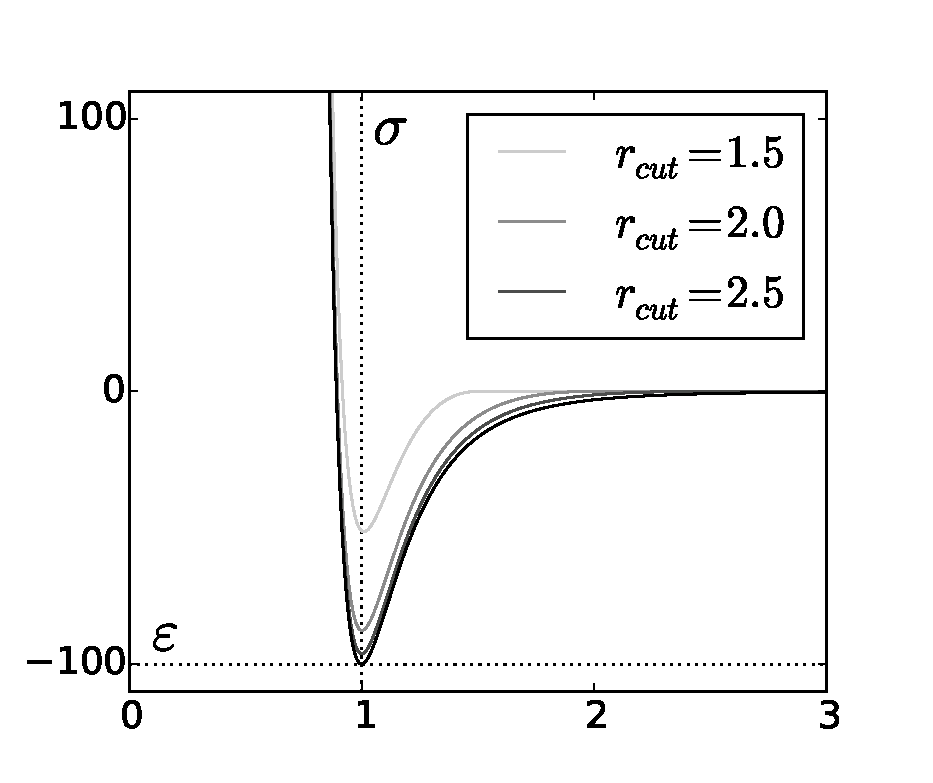
\includegraphics[scale=.5]{./fig/ch2/ljc_e.eps}
			\caption{Truncated Lennard-Jones energy. \label{subfig:LJTEnergy}}
		\end{subfigure}%
		~
		\begin{subfigure}[t]{.5\textwidth}
			\centering
			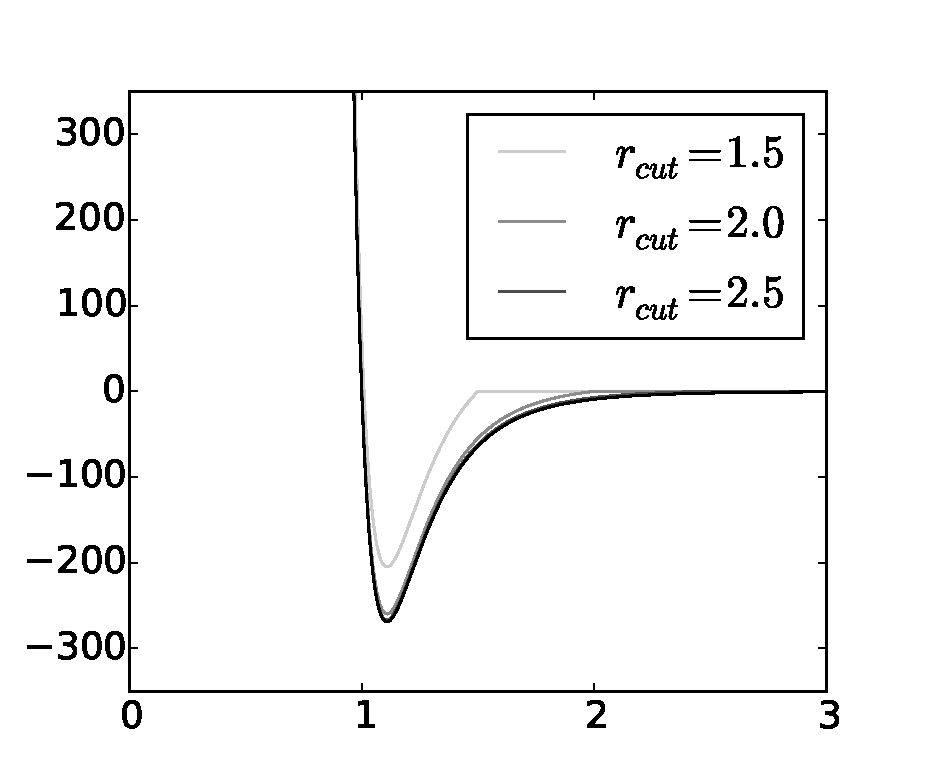
\includegraphics[scale=.5]{./fig/ch2/ljc_f.eps}
			\caption{Truncated Lennard-Jones force. \label{subfig:LJTForce}}
		\end{subfigure}		
		\caption{Lennard-Jones energy and force are in black in the respective figures as reference.\label{fig:LJT}}	
	\end{figure*}	

\noindent	
asymptotically approaches zero as $x$ approaches infinity. This makes Lennard-Jones a short range potential and, more importantly, makes interactions at long distances negligible. We can truncate (or cut) the potential at some radius $r_c$. However, this introduces a discontinuity in the potential, so in order to repair both the potential and it's derivative, we use the following modification,
\begin{equation}
	U_c(x; \varepsilon, \sigma) = \left\{ 
		\begin{array}{lr}
			U(x; \varepsilon, \sigma) - U(r_c; \varepsilon, \sigma) - \frac{dU}{dx}\bigg|_{x = r_c}(x - r_c), & x \leq r_c\\
			0, & x > r_c
		\end{array}
		\right. 
\end{equation}

	The sequence of truncated Lennard-Jones potentials converges to the Lennard-Jones potential as $r_c \to \infty$ and the truncated Lennard-Jones potentials share the same asymptotic behavior (see Figure~\ref{fig:LJT}). This truncation technique is referred to as shifted forces, it is commonly used to conserve energy in the potential and avoid potential artifacts with a model. The discontinuous truncation is also used but can cause larger discrepancies in energy particularly with very long simulations. Although this method alters the potential everywhere the accuracy with respect to the true potential has been observed in molecular dynamics simulations as better than the discontinuous truncation \cite{Toxvaerd2011}.
	
  Time dependent simulations leading to equilibrium for large systems can require long time intervals, so to avoid artifacts in the geometry we use the continuous variation of the truncated Lennard-Jones potential. Moreover, we pick a conservative cutoff selection of $r_c = 8$ in all simulations to further ensure accuracy of equilibrium configurations.

	In order to represent concisely the set of particles that a given particle is interacting with, we define the set
\begin{equation}
	P(j,i) = \{ (h,k)|j \neq h \vee k \neq i \pm 1, 1 \leq h \leq m, 1 \leq k \leq n_h \},
\end{equation}
which contains every particle that the $i$th particle on the $j$th fiber interacts with via the truncated 12-6 potential. Now we can express the vdW energy for the system,
\begin{multline}
	E_v = \sum_{j=1}^m \sum_{i=1}^{n_j} \bigg[ \sum_{(h,k) \in P(j,i)} U_c \left( \| \textbf{r}_i^{(j)} - \textbf{r}_k^{(h)} \|; \varepsilon, \sigma \right) \\ + \sum_{k=1}^{n_-} U_c \left( \| \textbf{r}_i^{(j)} - \textbf{r}_k^{(-)} \|; \varepsilon_-, \sigma \right) + \sum_{k=1}^{n_+} U_c \left( \| \textbf{r}_i^{(j)} - \textbf{r}_k^{(+)} \|; \varepsilon_+, \sigma \right) \bigg].
\end{multline}
It is not the case that the interaction strength is the same for each potential. There are different strengths for fiber to fiber, fiber to top substrate, and fiber to bottom substrate interactions.

% van der Waals lower substrate pressure
%\begin{equation}
%	E_p = \sum_{j=1}^m \sum_{i=1}^{en_j} U_p \left( y_i^{(j)} \right)
%\end{equation}

\subsection{Total energy}

With both springs and vdW interaction the system of fibers and the bottom substrate is complete. What is left is the rigid motion of the top substrate. We apply a load on the $0$th particle of the top substrate with vertical component $\lambda$ and horizontal component $\mu$. This is consistent with applying a load to the center of mass of the top substrate.

We have described the model so far as different partial energies. It comes as no surprise then that the total energy for the system is

% Total energy
\begin{equation}
	E = E_b + E_e + E_v + \lambda x_0^{(+)} - \mu y_0^{(+)}.
\end{equation}
The model for the system includes two springs, the extensible and torsional springs, the vdW interaction, and the rigid motion of the top substrate. Note that $\lambda$ is flipped from what might be considered intuition. Positive values of $\lambda$ will move the top substrate ``down'' towards the fiber, instead of ``up''.

\section{Dynamics}

Using Newton's second law with a damping term we have,

\begin{equation}
	M\frac{d^2\textbf{r}_i^{(j)}}{dt^2} + \frac{d\textbf{r}_i^{(j)}}{dt} = -\nabla_{\textbf{r}_i^{(j)}}E,
\end{equation}
for the $i$th particle on the $j$th fiber, where $M$ is the mass of the particle. We assume the mass of particles we want to take into consideration are small enough to make the acceleration negligible. This gives us,

\begin{equation}
	 \frac{d\textbf{r}_i^{(j)}}{dt} = -\nabla_{\textbf{r}_i^{(j)}}E.
\end{equation}
Approximating the derivative with a backwards difference gives us gradient descent,

\begin{equation}
    \textbf{r}_i^{(j),n} = \textbf{r}_i^{(j),n-1} - dt\nabla_{\textbf{r}_i^{(j)}}E.
\end{equation}
Clearly solving this ordinary differential equation will minimize the total energy.

The gradient flow dynamics of the governing equation have to be considered with the understanding that we assume our particles have sufficiently small mass. The model itself is abstract but it must be not be divorced from this assumption.

\section{Implementation}

   The implementation for the simulations that follow in Chapter~\ref{chap:three} and Chapter~\ref{chap:four} have a few implementation details that may be important to understand. We discuss those details here in order to give the reader a glimpse into what they might consider important factors in how to interpret results.

   The use of a truncated Lennard-Jones potential allows for an optimization that improves the average number of interactions that need to be computed. The optimization used in this work is a Verlet neighor list. However, using such a list leads to other important considerations, namely how it is to be updated. The trade off becomes an $\mathcal{O}(n)$ algorithm at each time step to determine if the list needs to be updated. Each time step the two largest displacements of unique particles are computed. If the sum of these displacements is larger than the buffer distance of the Verlet neighbor list then the list must be updated. The buffer zone in our case is the distance from our cutoff, $r_c = 8$, and a second cutoff, $r_{max} = 12$. For all simulations discussed here we have a buffer radius of $4$. Verlet neighbor lists are not the only manner of implementing the optimization and the reader may be interested in other solutions, such as cell lists.

   Equilibrium configurations are hard to decide on because we don't have infinite computation time to make sure nothing changes numerically. To ensure that the algorithm eventually stops we need an equilibrium criterion that when satisfied declares the system in equilibrium. In our case the equilibrium criterion is relative. That is, we take the norm distance between the current state vector and the prior state vector of the system. If this distance is less than a tolerance, $10^{-8}$, we mark the system as in equilibrium. However, we go one step further and require that this condition be satisfied persistently for ten time steps.

   There is another kind of equilibrium that is used to end early on simulations. If we have a load with negative or no vertical component, $\lambda$, then we likely only interested in how the top substrate interacts with the fibers of the system. If the top substrate is not interacting at all because it's too far away, then it is not coming back. That is, if the displacement of the top substrate $0$th particle is within $10^{-8}$ of it's maximum displacement, $\sqrt{\lambda^2 + \mu^2}$, then we say the system is in equilibrium. As before, this must hold for ten time steps before the simulation ends and the final decision is made.

   Finally, there are two versions of the code, MATLAB \cite{MATLAB2010} and C/C++. All results shown in this work use the C version only. However, the MATLAB version came first and the correctness of the C/C++ version was considered in relation to it. The software package used to evolve the system each time step was SUNDIALS, and in particular CVODE \cite{sundials}. All figures displayed in this work were generated using MatPlotLib \cite{Hunter2007}. The MATLAB and C/C++ simulation code, as well as the python visualization code are provided in appendices.

\chapter{Single fiber simulations} \label{chap:three}

We explore three experiments in the context of two substrates and one fiber of reasonable length ($n=96$). The first experiment, free standing, consists of the bottom substrate and a ``free standing'' fiber. Free standing in the sense that any buckled configuration for a set of parameters is not in principle caused by the load applied to the top substrate.

The second experiment, compression, adds the top substrate with some associated applied load. We measure the adhesion of particles of the fiber to particles of the top substrate and observe equilibrium configurations. The question of adhesion for these experiments is only relevant for a fiber particle in relation to a particle on one of the substrates. Thus we have the following heuristics,
\begin{eqnarray} \label{eqn:adhesion}
	A(\textbf{a}, \textbf{b}) = \left\{ 
		\begin{array}{ll}
			1, & \|\textbf{a} - \textbf{b}\| \leq 1.1 \sigma + 10^{-6}\\
			0, & \mbox{otherwise}
		\end{array}
		\right.  \\
	A_+ = \sum_{k=1}^{n^+} \sum_{j=1}^{m} \sum_{i=1}^{n} A(\textbf{r}_i^{(j)},\textbf{r}_k^{(+)}) \label{eqn:adhesion:top} \\ 
	A_- = \sum_{k=1}^{n^-} \sum_{j=1}^{m} \sum_{i=1}^{n} A(\textbf{r}_i^{(j)},\textbf{r}_k^{(-)}). \label{eqn:adhesion:bottom}
\end{eqnarray}
The equilibrium distance between any two particles is $\sigma$, however we relax this distance by $10\%$ and a numerical translation to take into account simulation precision.

The third experiment, detachment, consists of a fiber buckled only at the root and entirely adhered to both the top and bottom substrates. Adhered in the sense that every fiber particle will satisfy (\ref{eqn:adhesion}). A load is applied to the top substrate in an attempt to break an adhesive contact with the fiber. With all three experiments we focus primarily on equilibrium configurations. The heuristic (\ref{eqn:adhesion}) is then used as a method of categorizing different equilibrium configurations for varying parameters.

\section{Free standing}

We say a fiber, or part of a fiber, is \textit{crystallized} if the van der Waals energy between a collection of fiber particles appears qualitatively to be minimized. This is precisely the notion of adhesion we use for fiber particles in relation to substrate particles. Crystallization of a fiber is however a more global effect. If a fiber is going to crystallize at one location the same mechanism will cause crystallization elsewhere until several, if not all, particles on the fiber are in a crystallized state. 

	\begin{figure}[ht!]
		\begin{center}
			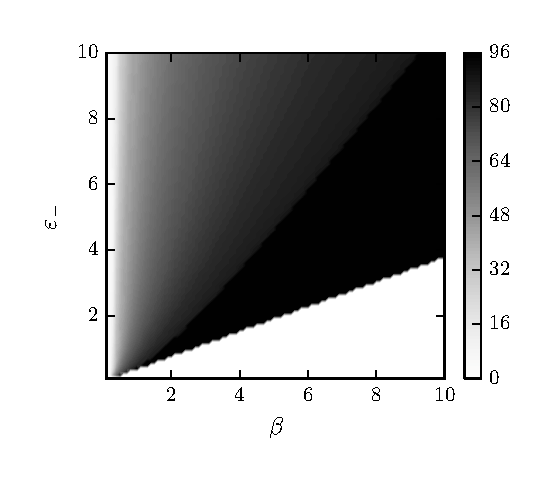
\includegraphics{./fig/ch3/fs/grid.eps}
		\end{center}		
		\caption{Plot of torsional spring strength, $\beta$, by bottom substrate vdW strength, $\eps_-$, colored by adhered (fiber) particle count to the bottom substrate. There are three distinct regions that categorize the behavior of a fiber: the black region of flattened fibers, the white region of standing or slanted fibers, and the grey sub-regions.
		\label{fig:fs}}
	\end{figure}

We say a fiber is \textit{flattened} if every particle of the fiber is adhered to the bottom substrate. If the parameters of the system are such that a fiber will be flattened in the free standing experiment then it would be difficult for the top substrate to have any influence on altering the fiber's configuration. In both the compression and detachment experiment we are more interested in parameters that do not give a flattened configuration. Therefore, it is pertinent to categorize for what parameters a fiber is flattened or not. In this regard we conjecture that the torsional spring and vdW interaction between the fiber and bottom substrate are critical and fiber to fiber vdW interaction or extensible springs are negligible.

	%% Fallen Figures
	\begin{figure*}[h!]
		\centering
		\begin{subfigure}{.5\textwidth}
			\centering
			\includegraphics{./fig/ch3/fs/b5_eb3.eps}
			\caption{$\beta=5$ and $\eps_-=3$.\label{subfig:lazy}}
		\end{subfigure}%
		~
		\begin{subfigure}{.5\textwidth}
			\centering
			\includegraphics{./fig/ch3/fs/b2_eb6.eps}
			\caption{$\beta=2$ and $\eps_-=6$.\label{subfig:lazy_loop}}
		\end{subfigure}

		\begin{subfigure}{.5\textwidth}
			\centering
			\includegraphics{./fig/ch3/fs/b0.5_eb10.eps}
			\caption{$\beta=0.5$ and $\eps_-=10$.\label{subfig:lazy_many_loops}}
		\end{subfigure}		
		\caption{The black region of Figure~\ref{fig:fs} consists strictly of (a) flattened fibers. (b) Configurations that contain a single kink are located in the grey region near the black region. (c) Configurations with additional kinks are located farther away.\label{fig:lazy}}	
	\end{figure*}

Varying $\beta$ and $\eps_-$ is shown in Figure~\ref{fig:fs} colored by fiber adhesion with the bottom substrate. The black region of the plot corresponds to flattened configurations, and only flattened configurations (see Figure~\ref{subfig:lazy}). If there is any buckling in the fiber a particle would be too far away to be considered adhered. 

	%% Erect Figures
	\begin{figure*}[t!]
		\centering
		\begin{subfigure}{.5\textwidth}
			\centering
			\includegraphics{./fig/ch3/fs/b10_eb1.eps}
			\caption{$\beta=10$ and $\eps_-=1$.\label{subfig:erect}}
		\end{subfigure}%
		~
		\begin{subfigure}{.5\textwidth}
			\centering
			\includegraphics{./fig/ch3/fs/b10_eb3.eps}
			\caption{$\beta=10$ and $\eps_-=3$.\label{subfig:leaning}}
		\end{subfigure}
		\caption{The white region of Figure~\ref{fig:fs} consists strictly of standing fibers. A standing fiber does not need to be (a) orthogonal to the bottom substrate, but can be (b) slanted and straight or curved.\label{fig:alert}}
	\end{figure*}

	%% Crystalized Figures
	\begin{figure*}[h!]
		\centering
		\begin{subfigure}{.5\textwidth}
			\centering
			\includegraphics{./fig/ch3/fs/b0.1_eb0.5.eps}
			\caption{$\beta=0.1$ and $\eps_-=0.5$.\label{subfig:hex_chain}}
		\end{subfigure}%
		~
		\begin{subfigure}{.5\textwidth}
			\centering
			\includegraphics{./fig/ch3/fs/b0.1_eb3.eps}
			\caption{$\beta=0.1$ and $\eps_-=3$.\label{subfig:leaning_hex_chain}}
		\end{subfigure}

		\begin{subfigure}{.5\textwidth}
			\centering
			\includegraphics{./fig/ch3/fs/b0.2_eb3.eps}
			\caption{$\beta=0.2$ and $\eps_-=3$.\label{subfig:crystal1}}
		\end{subfigure}%
		~
		\begin{subfigure}{.5\textwidth}
			\centering
			\includegraphics{./fig/ch3/fs/b0.2_eb9.eps}
			\caption{$\beta=0.2$ and $\eps_-=9$.\label{subfig:crystal2}}
		\end{subfigure}	
		\caption{Small $\beta$ of Figure~\ref{fig:fs} corresponds to fibers that crystallize with themself. Note the specific kind of crystallization of (a) and (b) as a pseudo-hexagonal chain configuration of the particles. Kinds of crystallization can be similar as with (c) and (d) but sutbly different.\label{fig:crystal}}	
	\end{figure*}

The white region of the plot consists of configurations were the fiber is either orthogonal to the bottom substrate, slanted but straight, or curved. In fact, we conjecture that a significant bend can only happen at the root, that all other particles are negligibly bent, and that if the root particle adheres to the bottom substrate then all particles will. Consider that the root particle of the fiber is nearest to the bottom substrate and will experience the strongest vdW interaction with the bottom substrate relative to any other fiber particle. If the vdW interaction causes the root particle torsional spring to bend but not buckle, then the force applied to the immediate next particle will be significantly smaller creating a negligible bend. If the vdW interaction is strong enough to cause the root particle to adhere to the bottom substrate then the torsional spring and the vdW interaction will move the next particle into an adhered state, and then the next, and so on. We observe from this argument a linear relationship between $\beta$ and $\eps_-$ at the dividing line between the white and black region. With sufficiently large $\beta$ relative to $\eps_-$ the fiber is not slanted (see Figure~\ref{subfig:erect}), and as $\beta$ decreases and $\eps_-$ increases, staying in the white region of Figure~\ref{fig:fs}, the fiber becomes more slanted (see Figure~\ref{subfig:leaning}).

They grey subregions of the plot are more complex and correspond to buckling at other particles of the fiber other than the root or fiber crystallization. Near the black region as $\eps_-$ is increased there is a gradual change from one buckle to two and so on. It appears that the particle at which buckles appear happen closer to the root with increased $\eps_-$ as well. The linear relationship between $\beta$ and $\eps_-$ is qualitative present between not only the white and black region, but the black and grey, and different grey shades. However, as $\beta$ decreases the slope increases. This trend hints that with smaller $\beta$ the fiber is more likely to crystallize. Crystallization for small $\beta$ is difficult to categorize with our adhesion heuristic, but Figure~\ref{fig:crystal} presents example crystallization configurations to help with our intuition. Most notably are configurations were the fiber can be said to be still ``standing'' as if the fiber to fiber vdW interaction has replace the torsional spring energy as a method of fiber stiffness (see Figure~\ref{subfig:hex_chain} and Figure~\ref{subfig:leaning_hex_chain}).

\section{Compression}

	\begin{table}[th]
		\rowcolors{1}{}{lightgray}
		\centering
		\caption{Reference parameters for compression.\label{table:compression_reference}}
		\begin{tabular}{lcrclcr}
			$m$ & = & 1 & \hspace{1in} & $\ell_-$ & = & 1 \\
			$n$ & = & 96 & & $\ell_+$ & = & 1 \\
			$n_+$ & = & 400 & & $\ell$ & = & 1 \\
			$n_-$ & = & 200 & & $\gamma$ & = & 100 \\
			$x^{(-)}$ & = & -100 & & $\beta$ & = & 10 \\
			$y^{(-)}$ & = & 0 & & $\eps_-$ & = & 1 \\
			$x^{(+)}$ & = & -200 & & $\eps_+$ & = & 1 \\
			$y^{(+)}$ & = & 110 & & $\eps$ & = & 1 \\
			$\delta$ & = & 0 & & $\sigma$ & = & 1
		\end{tabular}
	\end{table}
For the compression experiment a fiber is initially standing (see Figure~\ref{subfig:erect}). The primary focus is equilibrium configurations of the fiber under varying loads from the top substrate. Initially the top substrate is sufficiently far away from every particle on the fiber to prevent any vdW interaction, and because of this only loads with some nonzero positive vertical component are considered. A set of reference parameters in Table~\ref{table:compression_reference} are used in every case unless values are explicitly stated otherwise.

\subsection{Reference parameters}

	\begin{figure}[t]
		\begin{center}
			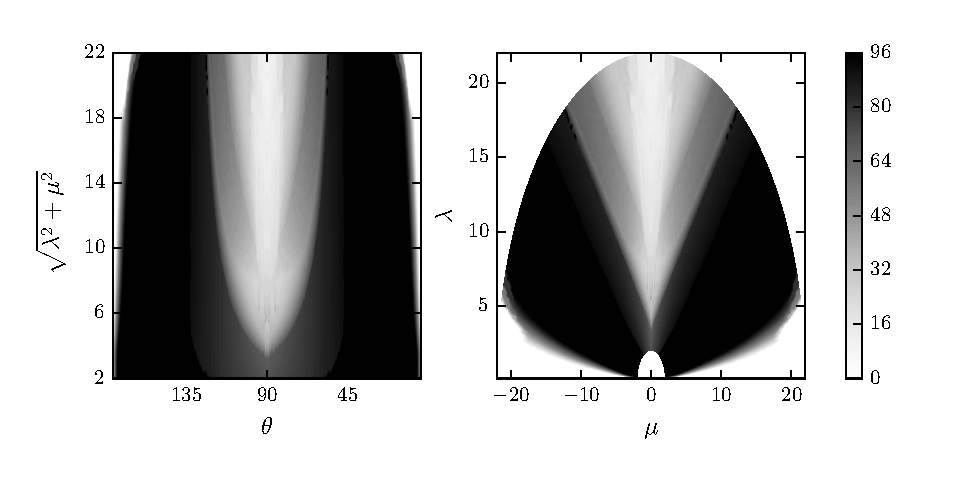
\includegraphics{./fig/ch3/push/ref/grid.eps}
		\end{center}		
		\caption{Plot of vertical component of load applied to the top substrate, $\lambda$, by the horizontal component, $\mu$, colored by adhered (fiber) particle count to the top substrate on the right. On the left is the same plot represented instead by the angle of the load by the load's magnitude colored in the same way. The black region consists of fibers that are in the \textit{flattened} configuration. There are obvious qualitative delineations of the plot by color but the categorization of the associated fiber configuration is not trivial.
		\label{fig:push:ref}}
	\end{figure}


Figure~\ref{fig:push:ref} plots the horizontal component of the load applied to the top substrate by it's vertical component colored by fiber particle adhesion to the top substrate. Analysis of contour plots of this nature will be the main focus of the results presented for the compression experiment. As with the free standing experiment, the black region of the plot corresponds to a flattened configuration as shown in Figure~\ref{subfig:flattened}. Indeed, for the contour plots of this kind throughout this section the black region will correspond to this and only this configuration. Aside from the black region there are other qualitative features of the plot: a white region, three distinct grey regions with sufficiently large magnitude of the load, small dark patches between two of those grey regions, and small grey patches in the white region for small magnitude of the load. We will explore the different regions of the plot through example.

For the darkest grey region we select $\lambda=14$ and $\mu=10.5$ as seen in Figure~\ref{subfig:flat_loop}. The configuration has one buckling point or \textit{kink}. A \textit{kink} is a buckle in a fiber that consists of relatively few particles and has sharp interior angles between bonds. This is contrast to what we consider a \textit{bend} in a fiber which consists of potentially many particles and small interior angles. For the darkest grey region we conjecture that as the angle of the load on the top substrate, $\theta$, is increased from $45$\textdegree the particle at which the kink in the fiber occurs will change to one further up the chain, thus causing less particles to be adhered.

	\begin{figure*}[h!]
		\centering
		\begin{subfigure}{.5\textwidth}
			\centering
			\includegraphics{./fig/ch3/push/ref/l5_m10.eps}
			\caption{$\lambda=5$ and $\mu=10$.\label{subfig:flattened}}
		\end{subfigure}%
		~
		\begin{subfigure}{.5\textwidth}
			\centering
			\includegraphics{./fig/ch3/push/ref/l14_m10.5.eps}
			\caption{$\lambda=14$ and $\mu=10.5$. \label{subfig:flat_loop}}
		\end{subfigure}

		\begin{subfigure}{.5\textwidth}
			\centering
			\includegraphics{./fig/ch3/push/ref/l15.5_m6.eps}
			\caption{$\lambda=15.5$ and $\mu=6$.\label{subfig:lonely_pancake}}
		\end{subfigure}%
		~
		\begin{subfigure}{.5\textwidth}
			\centering
			\includegraphics{./fig/ch3/push/ref/l19_m0.5.eps}
			\caption{$\lambda=19$ and $\mu=0.5$.\label{subfig:crushed}}
		\end{subfigure}
		\caption{Fiber configurations using the reference parameters in Table~\ref{table:compression_reference} with varying load. A contour plot of the adhered particle count is shown in Figure~\ref{fig:push:ref}. The black region of contour plot corresponds to (a) flattened fibers. They white region corresponds to configurations with (d) many folds. The grey region is complex and has different configurations two of which are shown in (b) and (c).\label{fig:ref_normal}}
	\end{figure*}

	\begin{figure*}[th!]
		\centering
		\begin{subfigure}{.5\textwidth}
			\centering
			\includegraphics{./fig/ch3/push/ref/l17_m11.eps}
			\caption{$\lambda=17$ and $\mu=11$.\label{subfig:tight_loop}}
		\end{subfigure}%
		~
		\begin{subfigure}{.5\textwidth}
			\centering
			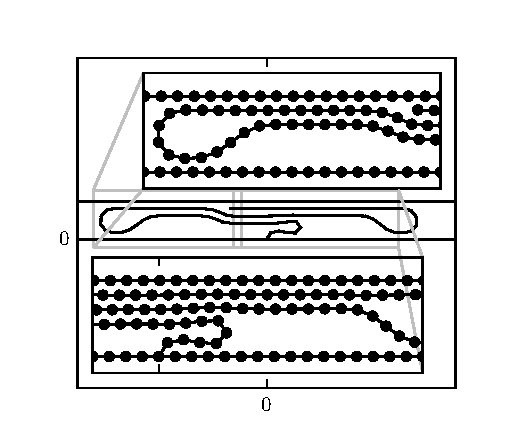
\includegraphics{./fig/ch3/push/ref/l5.9_m0.1.eps}
			\caption{$\lambda=5.9$ and $\mu=0.1$.\label{subfig:tight_hairpin}}
		\end{subfigure}
		\caption{Fiber configurations using the reference parameters in Table~\ref{table:compression_reference} with varying load. There are two locations in the contour plot of Figure~\ref{fig:push:ref} that are curious. There are patches of black between the whiter region and grey region of the plot (shown in (a)), and there are small grey pathces near the bottom of the white region (shown in (b)).\label{fig:ref_special}}
	\end{figure*}

The next darkest grey region does not have any observable difference between it and the following grey region. Configurations shown in Figure~\ref{subfig:lonely_pancake} or configurations very similar to it were observed in both regions of the plot. Although the pattern associated with the adhesion heuristic is not obvious it appears that with stronger vertical component, $\lambda$, the fiber contains more buckles (considering the same grey regions).

Figure~\ref{subfig:crushed} immediately describes the kinds of configurations that are found in the white region. The fiber is ``crushed'' underneath the load of the top substrate causing several kinks and bends. The mechanism in which some particles are able to adhere to the top substrate still while others are kept crystallized underneath the folds of the fiber itself is beyond the descriptive power of the adhesion heuristic. However, with variance in the white region in mind, equilibrium configurations are still likely to have the same ``crushed'' geometry.

Two special regions of the plot are the black patches between the darker two grey regions and the grey patches near $\theta=90$\textdegree and small magnitude of the load. We do not understand why these small regions appear. Figure~\ref{subfig:tight_loop} is an example of a configuration in the black patch region and Figure~\ref{subfig:tight_hairpin} is an example of a configuration in the grey patch region. Both configurations have bends in contrast to other configurations with similar loads with kinks.

	\begin{figure}[t]
		\begin{center}
			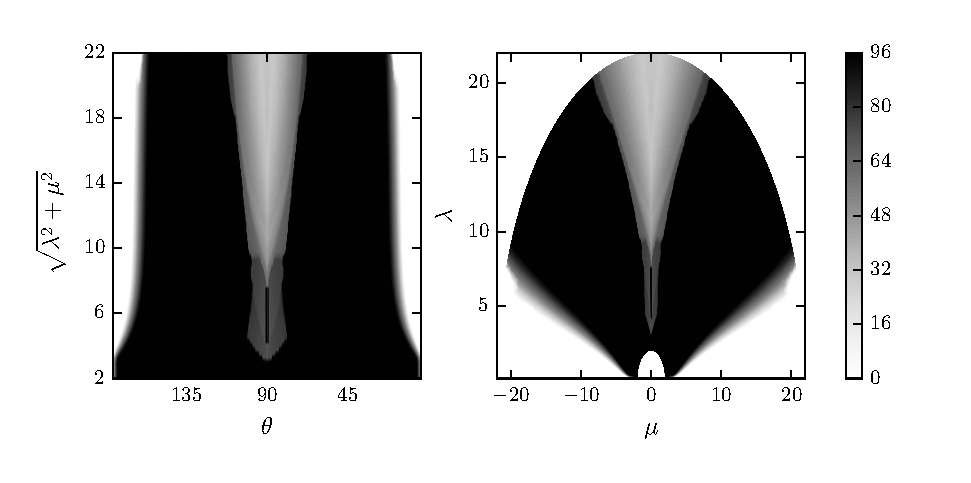
\includegraphics{./fig/ch3/push/b100/grid.eps}
		\end{center}		
		\caption{Plots of adhesive modes of a fiber under compression as in Figure~\ref{fig:push:ref}. Torsional spring strength is increased from reference parameters, $\beta=100$.
		\label{fig:push:b100}}
	\end{figure}	
	
	\begin{figure}[t]
		\begin{center}
			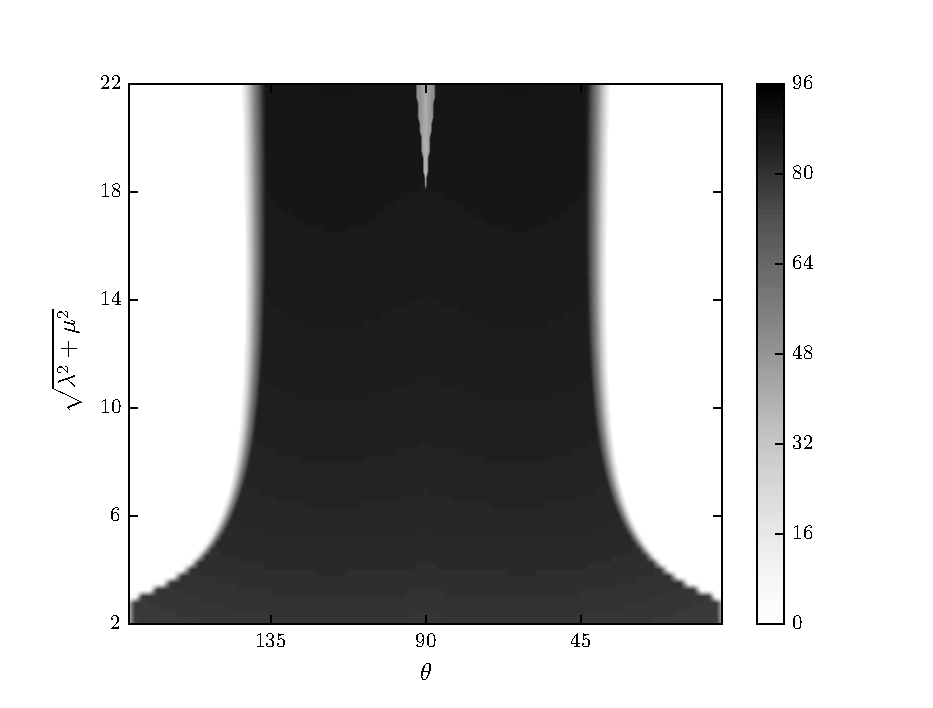
\includegraphics{./fig/ch3/push/b1000/grid.eps}
		\end{center}	
		\caption{Plots of adhesive modes of a fiber under compression as in Figure~\ref{fig:push:ref}. Torsional spring strength is increased from reference parameters, $\beta=1000$. The grey gradient from the top of the plot to the bottom immediately means that there is no strictly flattened fiber configuration.
		\label{fig:push:b1000}}
	\end{figure}
	
	\begin{figure*}
		\centering
		\begin{subfigure}{.5\textwidth}
			\centering
			\includegraphics{./fig/ch3/push/b100/l4.6_m0.65.eps}
			\caption{$\lambda=4.6$ and $\mu=0.65$.\label{subfig:short_loop}}
		\end{subfigure}%
		~
		\begin{subfigure}{.5\textwidth}
			\centering
			\includegraphics{./fig/ch3/push/b100/l19_m0.eps}
			\caption{$\lambda=19$ and $\mu=0$.\label{subfig:hairpin}}
		\end{subfigure}

		\begin{subfigure}{.5\textwidth}
			\centering
			\includegraphics{./fig/ch3/push/b1000/l3_m2.eps}
			\caption{$\lambda=3$ and $\mu=2$.\label{subfig:curved}}
		\end{subfigure}%
		~	
		\begin{subfigure}{.5\textwidth}
			\centering
			\includegraphics{./fig/ch3/push/b1000/l20_m0.eps}
			\caption{$\lambda=20$ and $\mu=0$.\label{subfig:long_loop}}
		\end{subfigure}	
		\caption{Fiber configurations using the reference parameters in Table~\ref{table:compression_reference}. Configurations (a) and (b) modify the reference paramters torsional spring string, $\beta=100$. Configurations (c) and (d) modify the same paramter, $\beta=1000$. From all configurations we note that an increase in $\beta$ correspondes to bends consisting of many particles instead of kinks consisting of few particles.\label{fig:bending_fiber}}	
	\end{figure*}

\subsection{Varying $\beta$}

The strength of the torsional spring strength, $\beta$, was shown as vitally important to a fiber moving to a flattened configuration or a standing one in Figure~\ref{fig:fs}. For the reference parameters in Table~\ref{table:compression_reference} $\beta$ is strong enough to stand freely. However, we are interested in significant modifications of the reference parameters by at least one order of magnitude. Decreasing the reference value of $\beta$ by an order of magnitude would make it too small for the fiber to stand freely. Because of this we only increase $\beta$.

Increasing $\beta$ by an order of magnitude such that $\beta=100$ significantly alters the picture from before. Shown in Figure~\ref{fig:push:b100} the black region of the plot is larger and grey and white regions have different shape. The difference in configurations for each region has much to do with precisely how many particles are part of a bend or if there is more than one bend. We present two examples: Figure~\ref{subfig:short_loop} corresponds to the black line inside the darker grey region, and Figure~\ref{subfig:hairpin} corresponds to $\theta=90$\textdegree with large magnitude.

The grey region of the contour plot is a similar configuration in Figure~\ref{subfig:short_loop} with the exception that more of the fiber is folded underneath itself causing a wave-like curve. The white regions also are similar to the example given in Figure~\ref{subfig:hairpin}. Even though there is variability in the heuristic it is because small numbers of particles are part of the curve of bends in the fiber instead of the adhered particles. This is the same idea shown in Figure~\ref{fig:push:ref} were slightly lighter portions of grey regions were because of configurations with a few particles being before instead of after the kink(s).

Increasing $\beta$ by another order of magnitude, $\beta=1000$, again significantly alters the picture. Figure~\ref{fig:push:b1000} shows the contour plot with this modification. Most notably is the loss of a black region, and a significantly smaller white region. The gradient of the grey region is represented in it's entirety with Figure~\ref{subfig:curved}. Any configuration in the grey region is only a fiber with a gradual bend from the root to the first adhered particle on the top substrate. This configuration is novel to $\beta=1000$ for the values we presented. The white region in contrast is similar to the same kind of configurations seen in the grey regions of $\beta=100$ with the exception of even more particles being in the bend (see Figure~\ref{subfig:long_loop}).

	\begin{figure}[t]
		\begin{center}
			\includegraphics{./fig/ch3/push/eb0.1/grid.eps}
		\end{center}		
		\caption{Plots of adhesive modes of a fiber under compression as in Figure~\ref{fig:push:ref}. VdW interaction strength of the bottom substrate is weakened, $\eps_-=0.1$.
		\label{fig:push:eb0.1}}
	\end{figure}	

	\begin{figure}[t]
		\begin{center}
			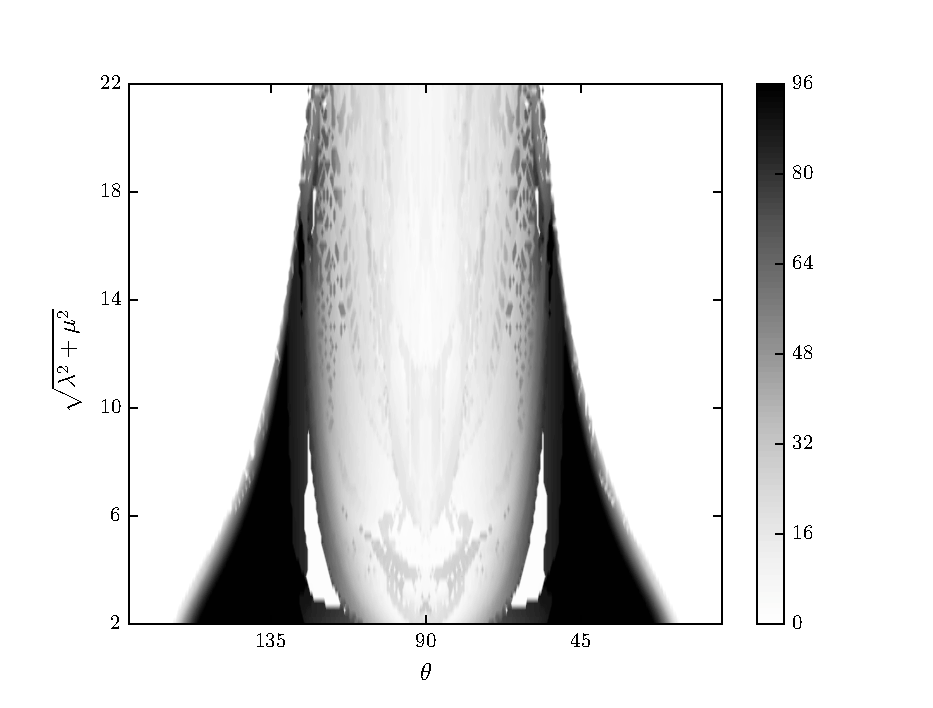
\includegraphics{./fig/ch3/push/et0.1/grid.eps}
		\end{center}		
		\caption{Plots of adhesive modes of a fiber under compression as in Figure~\ref{fig:push:ref}. VdW interaction strength of the top substrate is weakened, $\eps_+=0.1$. We note the dramatic change between this plot and Figure~\ref{fig:push:eb0.1} as they both are a weakening in vdW interaction by one order of magnitude.
		\label{fig:push:et0.1}}
	\end{figure}

	\begin{figure}[t]
		\begin{center}
			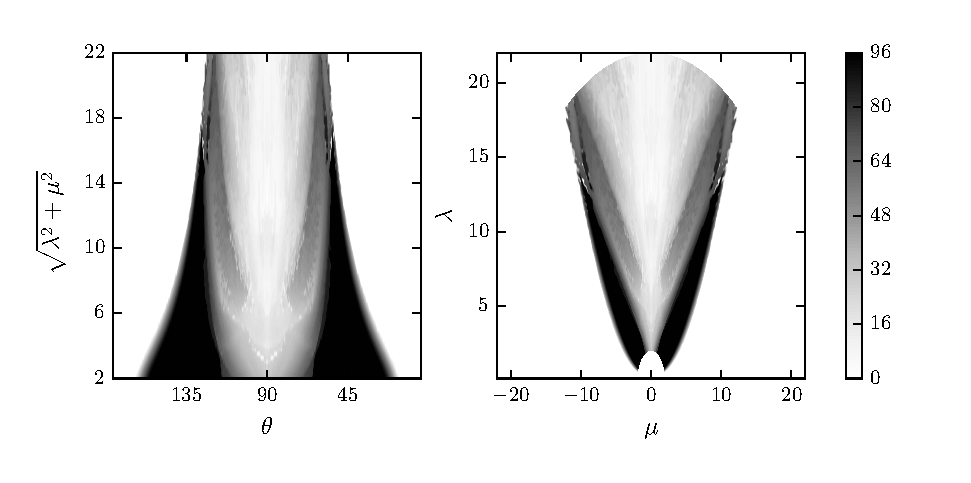
\includegraphics{./fig/ch3/push/eb0.1_et0.1/grid.eps}
		\end{center}		
		\caption{Plots of adhesive modes of a fiber under compression as in Figure~\ref{fig:push:ref}. VdW interaction strength of the top and bottom substrate is weakened, $\eps_+=0.1$ and $\eps_-=0.1$.
		\label{fig:push:eb0.1_et0.1}}
	\end{figure}	

	\begin{figure*}
		\centering
		\begin{subfigure}{.5\textwidth}
			\centering
			\includegraphics{./fig/ch3/push/eb0.1/l20.5_m3.5.eps}
			\caption{$\lambda=20.5$ and $\mu=3.5$.\label{subfig:multi_bridge}}
		\end{subfigure}%
		~
		\begin{subfigure}{.5\textwidth}
			\centering
			\includegraphics{./fig/ch3/push/eb0.1_et0.1/l20_m2.eps}
			\caption{$\lambda=20$ and $\mu=2$.\label{subfig:slant_crushed}}
		\end{subfigure}

		\begin{subfigure}{.5\textwidth}
			\centering
			\includegraphics{./fig/ch3/push/et0.1/l4.5_m1.eps}
			\caption{$\lambda=4.5$ and $\mu=1$.\label{subfig:bridge}}
		\end{subfigure}%
		~
		\begin{subfigure}{.5\textwidth}
			\centering
			\includegraphics{./fig/ch3/push/et0.1/l6_m4.eps}
			\caption{$\lambda=6$ and $\mu=4$\label{subfig:hump}}
		\end{subfigure}	
		\caption{Fiber configurations using the reference parameters in Table~\ref{table:compression_reference}. Configuration (a) modifies the reference paramters bottom substrate vdW interaction strength, $\eps_-=0.1$. Configuration (b) modifies the reference paramters bottom and top substrate vdW interaction strength, $\eps_-=0.1$ and $\eps_+=0.1$. Configurations (c) and (d) modify the reference parameters top substrate vdW interaction strength, $\eps_+=1$.\label{fig:vdw_crushed}}	
	\end{figure*}

\subsection{Varying $\eps_-$ and $\eps_+$} \label{subsection:push:eps}

Another method of allowing a fiber to stand instead of move to a flattened configuration is to decrease the vdW interaction strengths. Namely, we are interested in decreasing the vdW interaction strengths of both substrates, first independently and then together.

As a fiber is being compressed by the top substrate, it either began the process of adhering to the bottom substrate before the top substrate reaches it, or stands and is compressed strictly by the top substrate. For the reference parameters the fiber will begin to collapse on it's on, however not to a flattened configuration. Decreasing vdW interaction strength of the bottom substrate, $\eps_-=0.1$, will cause the fiber to be free standing. This modification means that the top substrate is the principal influence over how the fiber compresses, but after the fiber has been compressed the bottom substrate can stiffen the fiber's configuration. Figure~\ref{fig:push:eb0.1} shows the contour plot with this modification. Although there are noticeable differences the picture is qualitatively similar to the reference parameters picture, Figure~\ref{fig:push:ref}.

In contrast, when we decrease vdW interaction strength of the top substrate, $\eps_+=0.1$, the picture becomes significantly more complex (see Figure~\ref{fig:push:et0.1}). Previously we partitioned contour plots into regions using the adhesion heuristic as a guide. However, when we decrease vdW interaction strength the complexity in configurations becomes difficult to manage. Because of this difficulty we focus on specific features we can speak to, the overall comparison, and provide example configurations to give an intuition of the plots. In Figure~\ref{fig:push:et0.1} we have a white region for small magnitude of the load which corresponds to a ``hump'' configuration of the fiber (see Figure~\ref{subfig:hump}). As discussed before, because $\beta$ and $\eps_-$ are equal to the reference parameters the fiber will immediately begin to adhere to the bottom substrate. The top substrate vdW interaction strength is weaker which relaxes the constraints on the fiber both while it is being compressed and after it has been compressed. This allows for a kink to form near the root and for the fiber to completely adhere to the bottom substrate.

Decreasing vdW interaction strengths of both substrates to $0.1$ is shown in Figure~\ref{fig:push:eb0.1_et0.1}. With these modifications the primary modes of buckling involve parts of the fiber crystallizing. The grey region of the plot is similar to configurations shown in the reference parameters, specifically Figure~\ref{subfig:lonely_pancake}. The white region is also similar, consisting of ``crushed'' fiber configurations.

Example configurations for decreased vdW interaction strength are shown in Figure~\ref{fig:vdw_crushed}. These examples demonstrate some of the kinds of buckling that are exhibited but large categorizations of configurations as mentioned before difficult. With previous examples it was not wrong to assume, at least locally to the region in discussion, that the configurations were similar to the examples presented, but for these examples that is not necessarily true.
	
	\begin{figure}[t]
		\begin{center}
			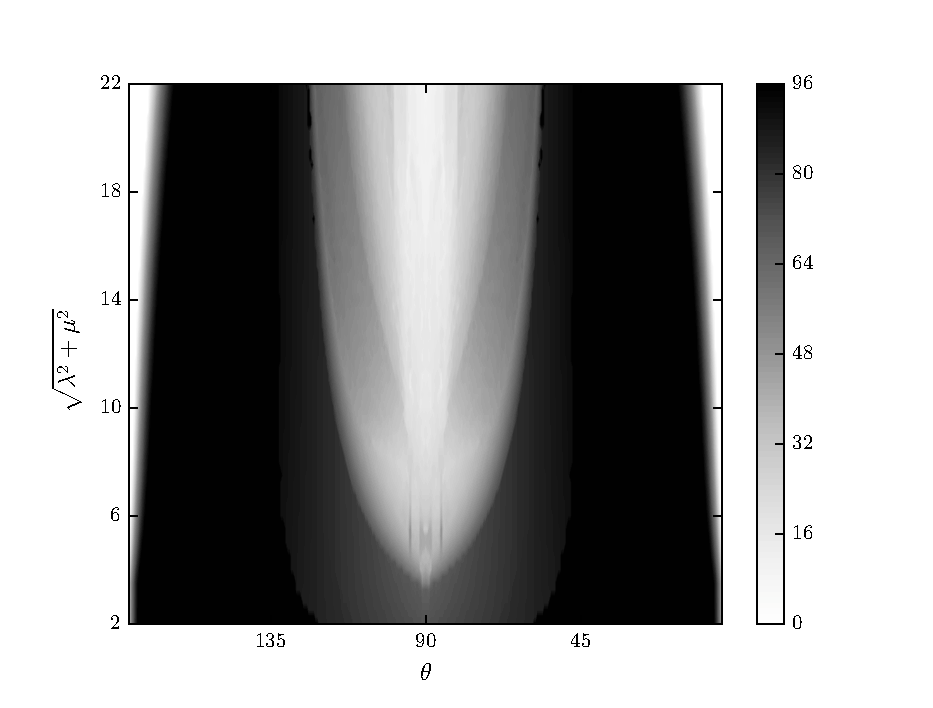
\includegraphics{./fig/ch3/push/g1000/grid.eps}
		\end{center}		
		\caption{Plots of adhesive modes of a fiber under compression as in Figure~\ref{fig:push:ref}. Extensible spring constant is increased, $\gamma=1000$.
		\label{fig:push:g1000}}
	\end{figure}	

\subsection{Varying $\gamma$}

We modify the extensible spring constant to ensure that our reference selecton, $\gamma=100$, is sufficiently large so that the fiber is sufficiently stiff. Figure~\ref{fig:push:g1000} for $\gamma=1000$ shows a contour plot similar to the reference plot (see Figure~\ref{fig:push:ref}). There are no qualitative differences between them which suggests that our selection of $\gamma$ is adequate.

	\begin{figure}[t]
		\begin{center}
			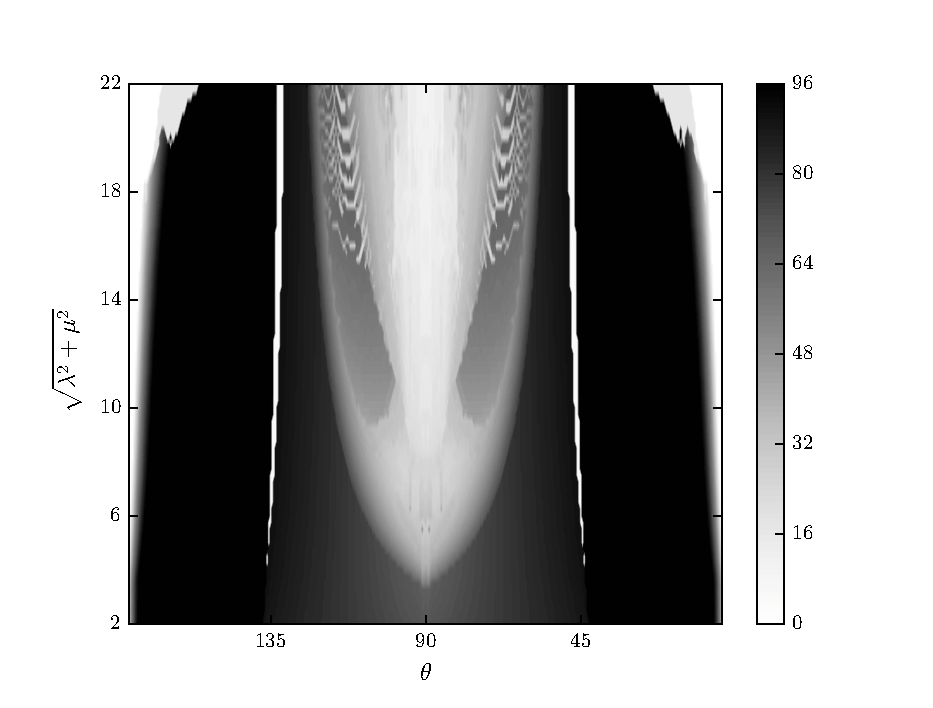
\includegraphics{./fig/ch3/push/p1/grid.eps}
		\end{center}		
		\caption{Plots of adhesive modes of a fiber under compression as in Figure~\ref{fig:push:ref}. The bottom substrate is replaced with a continuum of particles, that is the vdW interaction is integrated over the a bottom substrate of infinite length. The strength of the continuum vdW interaction is $p=1$.
		\label{fig:push:p1}}
	\end{figure}

\subsection{Bottom substrate with uniform potential} \label{section:compression:pressure}

A tangential curiosity is how the system behaves when the bottom substrate is a uniform potential instead of particle-particle potentials. We assume the bottom substrate is composed of infinitely many particles by integrating the Lennard-Jones potential. Every particle of the fiber interacts with the bottom substrate to this new uniform potential instead of a particle-particle potential.

Using the adhesion heuristic we see a similar picture to the reference parameters for the uniform potential (see Figure~\ref{fig:push:p1}). There are differences, most notably the white region of the plot between the black and dark grey regions. This region is the same kind of ``hump'' configuration we've seen before in Figure~\ref{subfig:hump}. Overall, we conjecture from both plots, Figure~\ref{fig:push:ref} and Figure~\ref{fig:push:p1}, that the different potentials give the same general behavior for the equilibrium configurations of the fiber, with some exceptions. This is however a limited comparison and those exceptions are not minor.

\section{Detachment} \label{ch:detachment}

In both the free standing and compression experiments we focused on a range of values of interest and presented a contour plot of the space using a heuristic for adhesion. With the detachment experiment we can explore the parameter space more intelligently. Instead of an exhaustive approach we assume that there is a critical magnitude of the load on the top substrate such that it will ``detach'' from the fiber. The top substrate is said to \textit{detach} from the fiber at the point in time when no particles of the fiber are adhered to the top substrate. If there is in fact a critical magnitude of the load for a given angle of the load then we can heuristically pick a sufficiently large magnitude such that the top substrate does detach and then bisect between that value and $0$. Note that the existence of a critical magnitude is not true in general and we will discuss such cases when they occur.

All simulations for the detachment experiment begin with the system in a flattened configuration (see Figure~\ref{subfig:flattened}). Although there are several compressed configurations from the previous experiment we focus on only the flattened configuration in this work.

	\begin{table}
		\rowcolors{1}{}{lightgray}
		\centering
		\caption{Reference parameters for the detachment experiment. \label{table:detachment_reference}}
		\begin{tabular}{lcrclcr}
			$m$ & = & 1 & \hspace{1in} & $\ell_-$ & = & 1 \\
			$n$ & = & 96 & & $\ell_+$ & = & 1 \\
			$n_+$ & = & 300 & & $\ell$ & = & 1 \\
			$n_-$ & = & 300 & & $\gamma$ & = & 100 \\
			$x^{(-)}$ & = & -150 & & $\beta$ & = & 1 \\
			$y^{(-)}$ & = & 0 & & $\eps^-$ & = & 1 \\
			$x^{(+)}$ & = & -150 & & $\eps^+$ & = & 1 \\
			$y^{(+)}$ & $\approx$ & 1.72741 & & $\eps$ & = & 1 \\
			$\delta$ & = & 0 & & $\sigma$ & = & 1
		\end{tabular}
	\end{table}
	
	\begin{figure}
		\begin{center}
			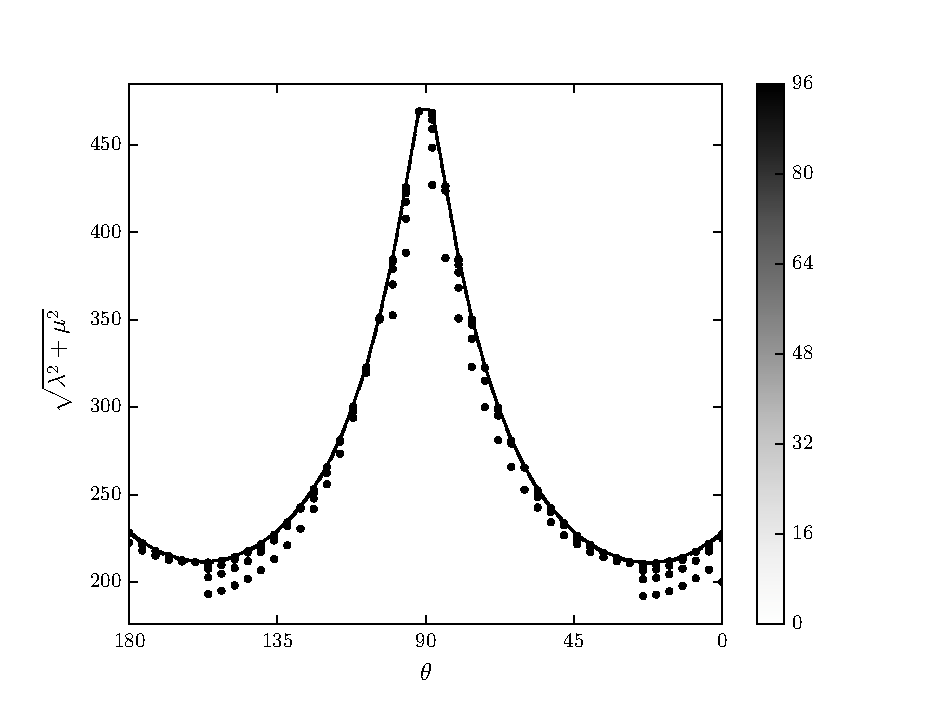
\includegraphics{./fig/ch3/pull/ref/grid.eps}
		\end{center}		
		\caption{The left is a plot of minimum critical load for the top substrate to detach from the fiber as function of the angle of the load. The right is the same plot in terms of the horizontal and vertical component of the load on the top substrate. For any given angle the critical load is only approximate, thus there are actually two lines drawn, one solid black representing the smallest detachment load, and a dashed line beneath it representing the largest adhesive load. Each circle represents a specific simulation.
		\label{fig:pull:ref}}
	\end{figure}

\subsection{Reference parameters}

As with the compression experiment we have a set of selected reference parameters in Table~\ref{table:detachment_reference}. Figure~\ref{fig:pull:ref} shows the critical magnitude for detachment of the load as a function of the angle of the load on the left, and the same line plotted via the components of the load on the right. There is a linear interpolation between every $4$th angle in the plot which makes determining maxima and minima to high absolute accuracy difficult but we are more interested in qualitative trends anyway. Every circle of the plot is a simulation for some specific value of $\lambda$ and $\mu$, and the color of the circle is the value of the adhesion metric between the fiber and the top substrate. All plots of the critical magnitude for detachment will follow these patterns.

Unlike the compression experiment, the detachment experiments do not yield as interesting equilibrium configurations. Above the critical magnitude in every case is a return to the free standing experiment with a different initial condition, and although that is interesting in it's own way the equilibrium configurations of those cases are not the focus of this experiment. Thus we ignore any simulations and configurations that happen above the critical magnitude. For the reference parameters, equilibrium configurations below the critical magnitude are all identical, they are the flattened configuration. Clearly the adhesion heuristic that has given us some success is not helpful in this case. In order to understand the picture then we turn to discussing the dynamics of the system under a detaching magnitude.

In the range $0 \leq \theta < 45$ the top substrate detaches from the fiber by sliding. The top substrate is said to ``slide'' if the particles on the top substrate shift from equilibrium with a collection of fiber particles to an equilibrium position with different collection of fiber particles in a finite amount of time. We conjecture there is a minimum in this range of $\theta$ values because there is an optimal angle of the load to maximize the number of particles are ``skipped'' when the top substrate slides across the fiber. As the angle of the load increases the effective horizontal distance traveled is reduced instead of improved.

Considering the range $45 \leq \theta < 90$ the top substrate continues the sliding mode of detachment up until what is assumed to be a critical angle where the effective horizontal displacement of a single particle on the top substrate is too small to slide over a single particle of the fiber. At this critical angle the mode of detachment changes from sliding to brute force. The top substrate is said to detach from the fiber via ``brute force'' if the critical magnitude of the load must be large enough to break every vdW interaction between the fiber and the top substrate simultaneously.

The range $90 \leq \theta \leq 180$ is similar. There is a critical angle of the load such that the top substrate changes from detaching from the fiber via brute force to detaching from the fiber by sliding, and there is a minimum angle of the load such that the displacement of a given particle on the top substrate is maximized during sliding. However, the way in which sliding occurs is subtly different. There is an observable asymmetry in the plot which is not fully understood. One explanation is that if the top substrate pulls against the direction that the fiber has been flattened (in this case to the right) then the torsional spring energy will push a particle of the fiber up into the top substrate repelling it from the fiber and thus making it easier to slide.

The plot on the right of Figure~\ref{fig:push:ref} tells the same story from a different perspective. With it we can see that the critical load is a linear relationship between the components of the load $\lambda$ and $\mu$ on either side of$\theta=90$\textdegree . 

	\begin{figure}[t]
		\begin{center}
			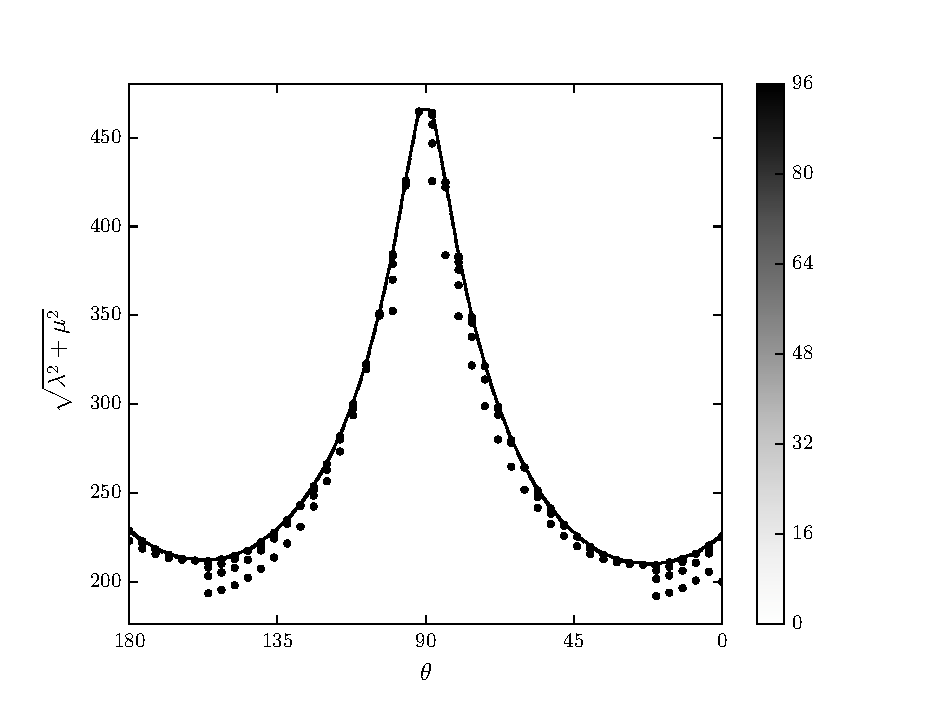
\includegraphics{./fig/ch3/pull/b10/grid.eps}
		\end{center}		
		\caption{Plot of the minimum critical magnitude for detachment as in Figure~\ref{fig:pull:ref}. The torsional spring strength is increased, $\beta=10$, from the reference parameters in Table~\ref{table:detachment_reference}.
		\label{fig:pull:b10}}
	\end{figure}
	
	\begin{figure}[t]
		\begin{center}
			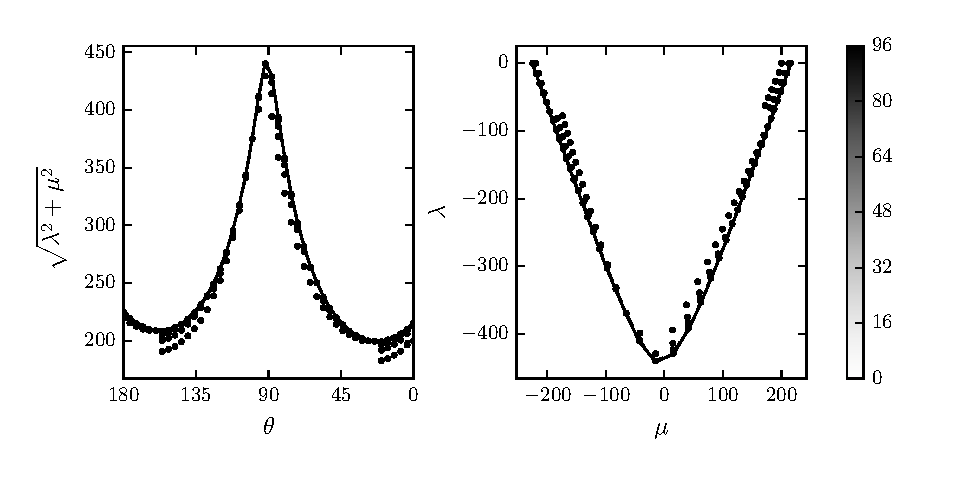
\includegraphics{./fig/ch3/pull/b100/grid.eps}
		\end{center}		
		\caption{Plot of the minimum critical magnitude for detachment as in Figure~\ref{fig:pull:ref}. The torsional spring strength is increased, $\beta=100$.
		\label{fig:pull:b100}}
	\end{figure}
	
\subsection{Varying $\beta$}

For the compression experiment $\beta$ was already sufficiently large for a fiber to stand freely. In the case of the detachment experiment $\beta=1$ is a magnitude lower and the fiber will not be able to stand freely. Like before, with the same reasoning, we focus only on increasing $\beta$.

With increased $\beta$ the story does not signficantly change. Figure~\ref{fig:pull:b10} and Figure~\ref{fig:pull:b100} show plots that are similar in general shape to the reference parameters. When the dynamics of a detachment are observed they are also very similar to the reference parameters. However, the values of extrema are different with larger $\beta$. The local minimum of the critical detachment load to the left of the maximum value is larger as $\beta$ increases. In contrast, the minimum value to the right of the maximum value of smaller as $\beta$ increases. This means the asymmetry in the plot is more exaggerated with larger $\beta$. This observation is consistent with the given explanation for the asymmetry being related to torsional springs near the root particle of the fiber. Lastly, the maximum critical magnitude decreases as $\beta$ increases.

	\begin{figure}
		\begin{center}
			\includegraphics{./fig/ch3/pull/eb0.1/grid.eps}
		\end{center}		
		\caption{Plot of the minimum critical magnitude for detachment as in Figure~\ref{fig:pull:ref}. The strength of the vdW interaction for the bottom substrate is decreased, $\eps_-=0.1$. In both plots there is a black star marker which corresponds to a detachment magnitude that happens below what we consider the critical magnitude.
		\label{fig:pull:eb0.1}}
	\end{figure}

	\begin{figure}
		\begin{center}
			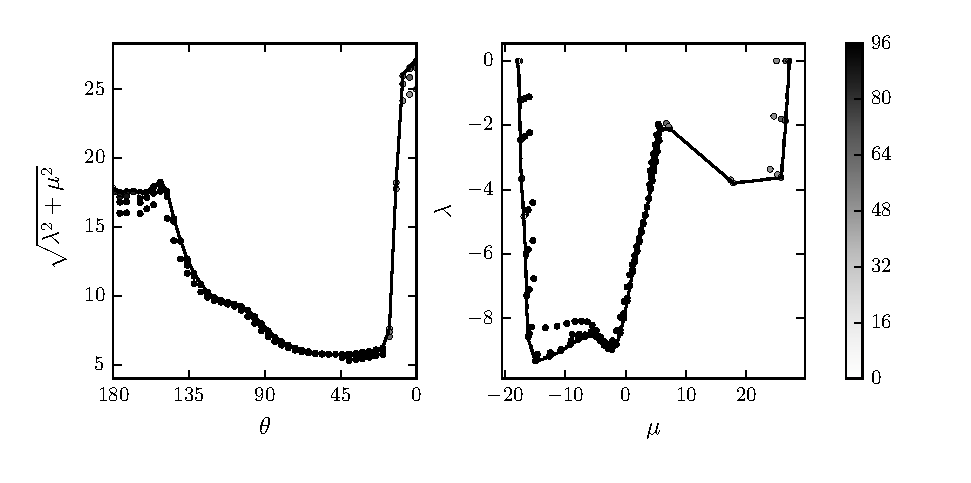
\includegraphics{./fig/ch3/pull/eb0.01/grid.eps}
		\end{center}		
		\caption{Plot of the minimum critical magnitude for detachment as in Figure~\ref{fig:pull:ref}. The strength of the vdW interaction for the bottom substrate is decreased, $\eps_-=0.01$. 
		\label{fig:pull:eb0.01}}
	\end{figure}
	
	\begin{figure}
		\begin{center}
			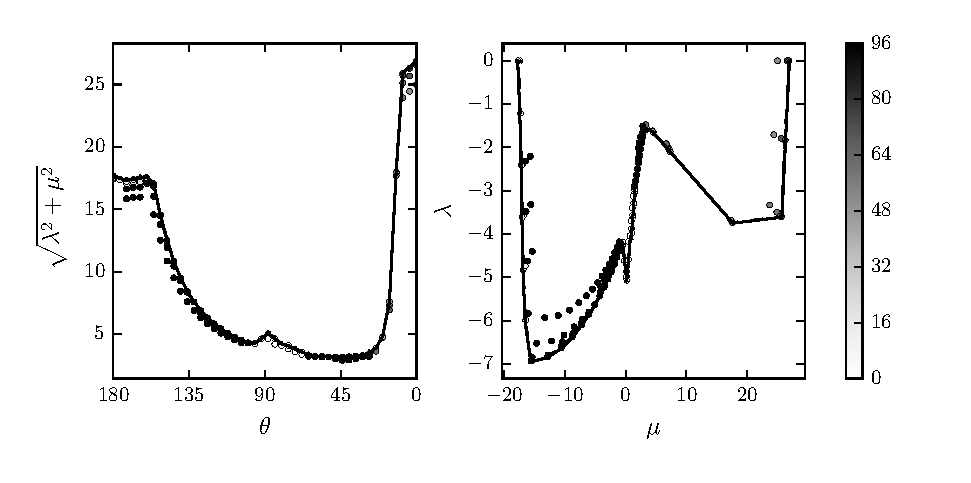
\includegraphics{./fig/ch3/pull/eb0/grid.eps}
		\end{center}		
		\caption{Plot of the minimum critical magnitude for detachment as in Figure~\ref{fig:pull:ref}. The strength of the vdW interaction for the bottom substrate is removed, $\eps_-=0$. Note that simulation circles that are white are not the same as star markers representing isolated detachments.
		\label{fig:pull:eb0}}
	\end{figure}
	
	\begin{figure}
		\begin{center}
			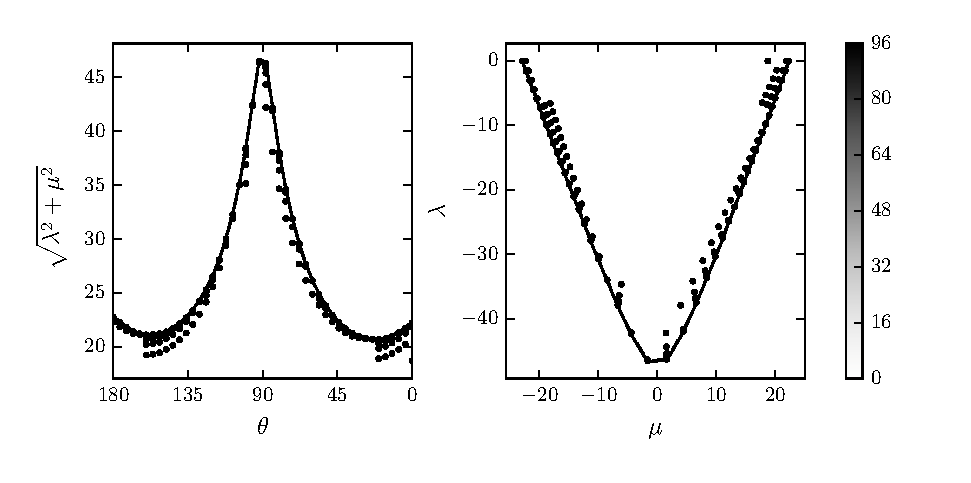
\includegraphics{./fig/ch3/pull/eb0.1_et0.1/grid.eps}
		\end{center}		
		\caption{Plot of the minimum critical magnitude for detachment as in Figure~\ref{fig:pull:ref}. The strength of the vdW interaction for the bottom and top substrate are decreased, $\eps_-=0.1$ and $\eps_+=0.1$.
		\label{fig:pull:eb0.1_et0.1}}
	\end{figure}
	
	\begin{figure}
		\begin{center}
			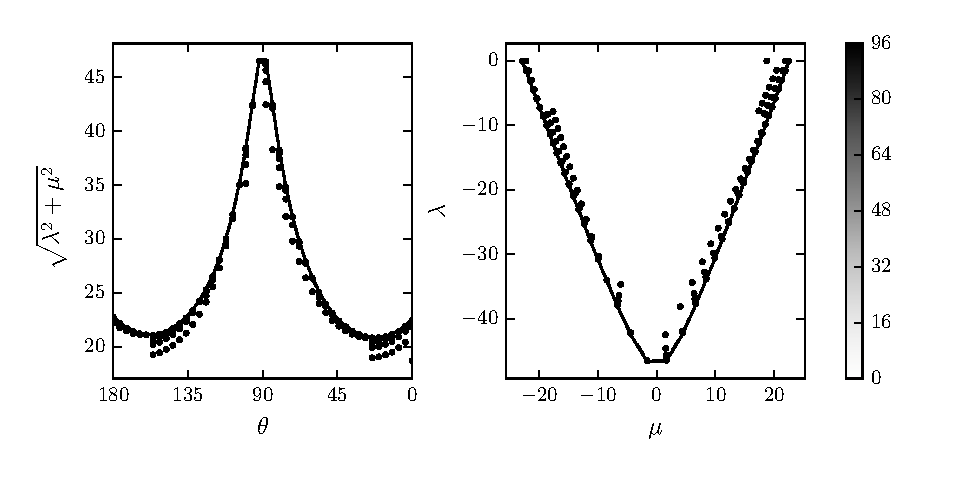
\includegraphics{./fig/ch3/pull/eb0.1_et0.1_e0.1/grid.eps}
		\end{center}		
		\caption{Plot of the minimum critical magnitude for detachment as in Figure~\ref{fig:pull:ref}. The strength of the vdW interaction for all particles are decreased, $\eps_-=0.1$, $\eps_+=0.1$, and $\eps=0.1$.
		\label{fig:pull:eb0.1_et0.1_e0.1}}
	\end{figure}
	
	\begin{figure}
		\begin{center}
			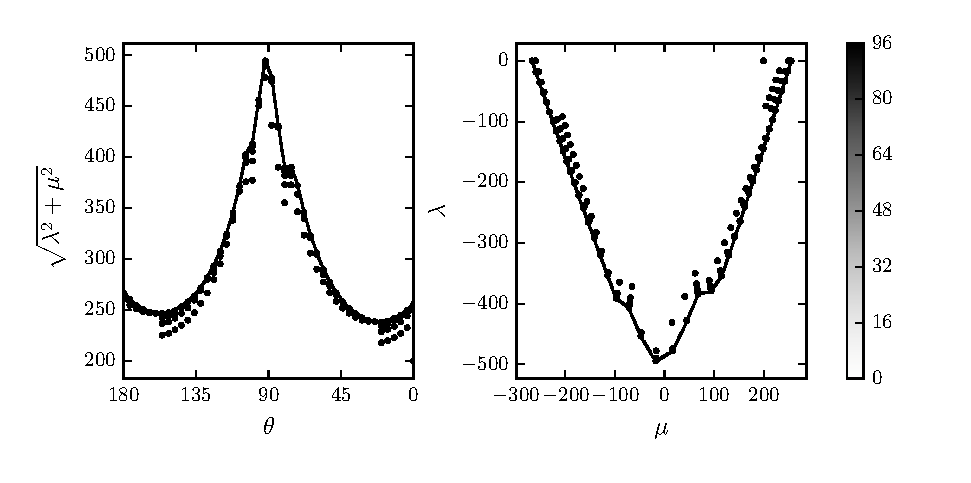
\includegraphics{./fig/ch3/pull/et10/grid.eps}
		\end{center}		
		\caption{Plot of the minimum critical magnitude for detachment as in Figure~\ref{fig:pull:ref}. The strength of the vdW interaction for the top substrate is increased, $\eps_+=10$.
		\label{fig:pull:et10}}
	\end{figure}

\subsection{Varying $\eps^-$, $\eps^+$, and $\eps$} \label{section:detachment:eps}

Varying vdW interaction strengths has the most significant effect on the results of the detachment experiment that we have observed. First, we consider decreasing $\eps_-$ and $\eps_+$ to $0.1$ and related all three vdW interactions, $\eps_- = \eps_+ = \eps = 0.1$. Second, we consider the case were only $\eps_-=0.1$ and the case where only $\eps_+=10$. Lastly, we consider decreasing $\eps_-$ further, exploring both $\eps_-=0.01$ and $\eps_-=0$.

For $\eps_- = \eps_+ = 0.1$ the critical magnitude for detachment is decreased for all angles of the load by approximately an order of magnitude. Figure~\ref{fig:push:eb0.1_et0.1} demonstrates the linear relationship between the critical detachment load and vdW uniform decrease in the substrate interaction strengths. However, the modes of detachment are significantly different. 


For the same reason we only increase $\beta$, here we only decrease the vdW interaction strengths. Our first interest is in decreasing $\eps^-$ only. Here we notice an exception in the assumptions we've used so far. An \textit{isolated detachment} is a load that will cause the upper substrate to detach from the fiber even though with a small increase in magnitude the substrate would stay adhered. The reasons for this have much to do with the propagating wave and how the upper substrate's particles align with the fiber's particles. Even one reduction in order of magnitude of $\eps^-$ has a significant qualitative effect (see Figure~\ref{fig:PullGrid:eb0.1}). The magnitude required for the upper substrate to detach is significantly less for every angle. Moreover, although the general symmetry survives to a certain point there are significantly more asymmetries. As $\eps^-$ is reduced by another order of magnitude the picture changes entirely as we can see from Figure~\ref{fig:PullGrid:eb0.01}. With the adhesion between the fiber and the bottom substrate so significantly weakened the reinforcement of the flattened state is removed and allows for the upper substrate to zip free of the fiber one vdW bond at a time. Thus, the initial resistance in moving the root and causing a propagating wave is no longer the primary method of detachment and becomes the greatest hindrance instead. When $\eps^-$ is reduced to the point of vanishing this zipping around no shear component becomes more obvious as magnitude just slightly below the minimum has only one particle adhered to the upper substrate (see Figure~\ref{fig:PullGrid:eb0}). It would seem then that zipping is an efficient enough method of detachment that it is easier to zip free of a bond than it is to break one. The resistance when there is primarily only a shear component again has the same difficulty as before.

In Figure~\ref{fig:PullGrid:eb0.1_et0.1} we reduce both $\eps^-$, and $\eps^+$ by an order of magnitude. In comparison to the reference parameters the major difference is in the required magnitude to detach. This would seem like the obvious consequence as vdW bonds are the only reason for attachment. In Figure~\ref{fig:PullGrid:eb0.1_et0.1_e0.1} $\eps$ is also reduced by an order of magnitude, but there is no qualitative difference between the two. We also increase just $\eps^+$ in one case (see Figure~\ref{fig:PullGrid:et10}). We can see from the figure that it is most directly comparable to Figure~\ref{fig:PullGrid:eb0.1}.

	\begin{figure}
		\begin{center}
			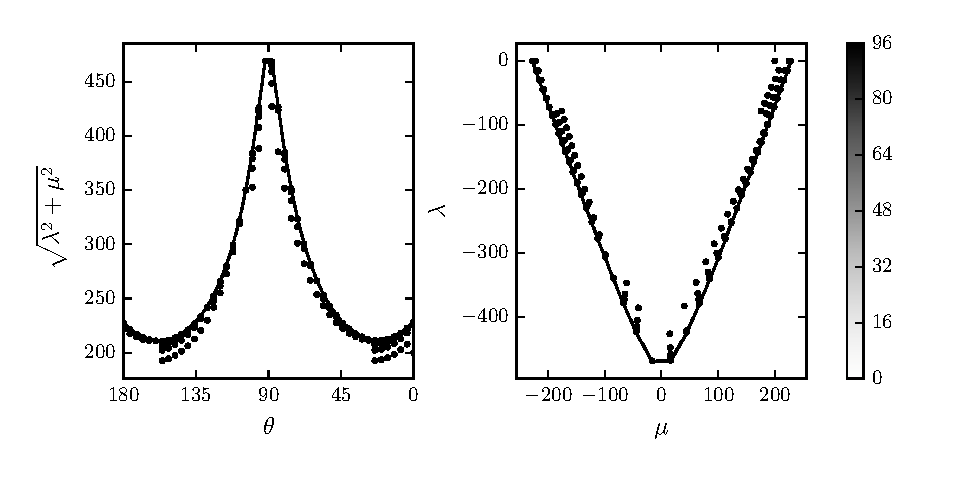
\includegraphics{./fig/ch3/pull/g1000/grid.eps}
		\end{center}		
		\caption{Plot of the minimum critical magnitude for detachment as in Figure~\ref{fig:pull:ref}. The extensible spring constant is increased, $\gamma=1000$.
		\label{fig:pull:g1000}}
	\end{figure}

\subsection{Varying $\gamma$}

We modify the extensible spring constant to ensure the reference selection, $\gamma=100$, is sufficiently stiff. Although larger values of $\gamma$ will alter the dynamics and equilibrium configurations we want extensible springs to be able to relax without significant changes between results with our selected value and larger values. Figure~\ref{fig:pull:g1000} shows the plot of the critical magnitude of the load. The similarity between this plot and the reference plot in Figure~\ref{fig:pull:ref} suggests our selection of $\gamma$ is sufficient.

	\begin{figure}
		\begin{center}
			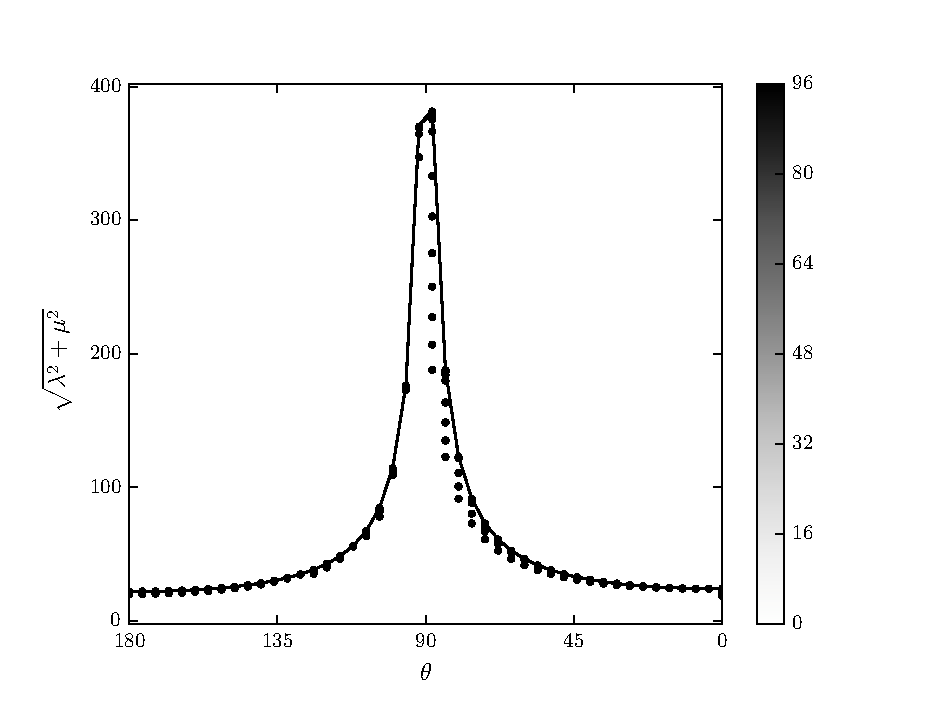
\includegraphics{./fig/ch3/pull/p1/grid.eps}
		\end{center}		
		\caption{Plot of the minimum critical magnitude for detachment as in Figure~\ref{fig:pull:ref}. The bottom substrate is replaced with a continuum of particles, that is the vdW interaction is integrated over the entire real line. The strength of the continuum vdW interaction is $p=1$.
		\label{fig:pull:p1}}
	\end{figure}
	
	\begin{figure}
		\begin{center}
			\includegraphics{./fig/ch3/pull/p10/grid.eps}
		\end{center}		
		\caption{Plot of the minimum critical magnitude for detachment as in Figure~\ref{fig:pull:ref}. The bottom substrate is replaced with a continuum of particles. The strength of the continuum vdW interaction is $p=10$.
		\label{fig:pull:p10}}
	\end{figure}

\subsection{Bottom substrate with uniform potential} \label{section:detachment:pressure}

In section~\ref{section:compression:pressure} we replaced the bottom substrate particle-particle potential with a uniform potential. We make the same modification here and briefly discuss the effects on the model under the detachment experiment.

Figure~\ref{fig:pull:p1} and Figure~\ref{fig:pull:p10} show the critical magnitude of the load with the modified bottom substrate potential. The dynamics of the detachment situation are the same as the reference parameters, i.e. that there are two detachment modes: sliding and brute force. There is still a maximum of the critical load near $\theta=90$\textdegree ~and still likely a critical angle were the detachment mode changes. However, the minimums on either side of the plot have changed. An explanation is that there is no resistance for the fiber particles to prevent horizontal displacement because the potential is uniform. Any vertical component of the load does not assist the top substrate in detaching from the fiber which means the minimums on the left and right of the plot should be at $\theta=0$ and $\theta=180$.

	\begin{figure*}
		\centering
		\begin{subfigure}{.5\textwidth}
			\centering
			\includegraphics{./fig/ch3/pull/eb0.1/l0_m32.8.eps}
			\caption{$\lambda=0$ and $\mu=32.8$. \label{subfig:folded_over}}
		\end{subfigure}%
		~
		\begin{subfigure}{.5\textwidth}
			\centering
			\includegraphics{./fig/ch3/pull/eb0/t76_m4.eps}
			\caption{$\lambda\approx3.88$ and $\mu\approx0.968$\label{subfig:barely_adhered}}
		\end{subfigure}
		\caption{Configuration (a) is an archetypal example of angles of loads on the top substrate that are close to 0. Such loads will often fold ontop of themselves as the top substrate pulls them to the right. Configuration (b) is an archetypal example of the white simulations in the plot for Figure~\ref{fig:pull:eb0}. The reference parameters are modified differently in both examples, for (a) $\eps_-=0.1$ and for (b) $\eps_-=0$.\label{fig:pull_equil}}	
	\end{figure*}

	\begin{figure*}
		\centering
		\begin{subfigure}{.5\textwidth}
			\centering
			\includegraphics{./fig/ch3/pull/unzip_anim.eps}
			\caption{\label{subfig:unzip}}
		\end{subfigure}%
		~
		\begin{subfigure}{.5\textwidth}
			\centering
			\includegraphics{./fig/ch3/pull/wave_anim.eps}
			\caption{\label{subfig:travel_waves}}
		\end{subfigure}
		\caption{Three time steps of a moving fiber as examples for the kinds of detachemnt modes. Darker fibers are later in the evolution of time. For (a) we see an unzipping mode of detachment were a the top substrate and fiber break the vdW interaction between one particle at a time. For (b) wee see a propogation of waves through a fiber.\label{fig:animation}}	
	\end{figure*}
	
\chapter{Many fiber simulations} \label{chap:four}

	\begin{table}
		\rowcolors{1}{}{lightgray}
		\centering
		\caption{Reference parameters for all simulations presented in this chapter. Note that $n_j$ and $\delta_j$ are functions of $j$. For each $j$, $n_j$ is constant and $\delta_j$ is linear. \label{table:manyfiber_reference}}
		\begin{tabular}{lcrclcr}
			$m$ & = & 10 & \hspace{1in} & $\ell_-$ & = & 1 \\
			$n_j$ & = & 96 & & $\ell_+$ & = & 1 \\
			$n_+$ & = & 360 & & $\ell$ & = & 1 \\
			$n_-$ & = & 310 & & $\gamma$ & = & 100 \\
			$x^{(-)}$ & = & -110 & & $\beta$ & = & 10 \\
			$y^{(-)}$ & = & 0 & & $\eps_-$ & = & 0.1 \\
			$x^{(+)}$ & = & -160 & & $\eps_+$ & = & 1 \\
			$y^{(+)}$ & = & 110 & & $\eps$ & = & 0.1 \\
			$\delta_j$ & = & 10$j$ & & $\sigma$ & = & 1
		\end{tabular}
	\end{table}

	In Chapter~\ref{chap:three} we discussed three different simulation experiments: a fiber standing free of load, a fiber under compression from the top substrate, and the top substrate detaching from the fiber. Here we look at the compression experiment with ten fibers. As before we have a set of reference parameters (see Table~\ref{table:manyfiber_reference}). We run the compression experiment on the reference parameters and three variations of the parameters, specifically varying $\beta$, $\gamma$, and $\eps_+$.

	\begin{figure}
		\begin{center}
			\includegraphics[scale=1]{./fig/ch4/grid.eps}
		\end{center}		
		\caption{Equilibrium configurations of ten fibers with 96 particles each for varying loads. The top left plot is a configuration with a load of $\lambda = 5$ and $\mu = 0$. The configurations immediately to the right are increasing $\mu$, and immediately below are increasing $\lambda$. All configurations use the reference parameters in Table~\ref{table:manyfiber_reference}.
		\label{fig:grid}}
	\end{figure}
	
	For computational reasons the granularity of our search space is signficantly smaller than with the single fiber case. We consider nine simulations with values of $\lambda = 5, 15, 25$ and $\mu = 0, 5, 10$. In Figure~\ref{fig:grid} we see a high level view of each simulation for the reference parameters. Keeping the horizontal component of the load zero, we see an increase in the aggregate curvature of all ten fibers as we increase $\lambda$. One explanation for this is that the torsional and extensible springs are not given enough leverage to slide along the top substrate and align to it. As the magnitude of the load is increased the fibers become more likely to buckle. If we increase $\mu$ the story changes. We are able to maintain the aligned compressed configuration for larger magnitudes of the load if the horizontal component is sufficiently large. It would seem the ratio between vertical and horizontal component for the reference parameters is the deciding factor for whether or not fibers will buckle.

	\begin{figure}
		\begin{center}
			\includegraphics[scale=1]{./fig/ch4/grid_b100.eps}
		\end{center}		
		\caption{Equilibrium configurations of varying loads. All configurations are directly comparable to Figure~\ref{fig:grid} with the exception that $\beta = 100$.
		\label{fig:grid_b100}}
	\end{figure}

	In Figure~\ref{fig:grid_b100} we increase $\beta$ to one hundred. This is an order of magnitude increase from the reference parameters and prevents any buckling at all for the loads we have selected. Qualitatively it is hard to see any difference in any of the nine simulations with the one exception that the fibers buckle to the left with no horizontal component. This bias with a load that has no horizontal component could be caused by a numerical artifact or an asymmetry in the number of atoms on the top substrate to the left of the leftmost fiber versus to the right of the rightmost fiber. Regardless of the reason the configuration itself is close enough to a reflection of the other configurations with a nonzero horizontal component that it would seem negligible.
	
	\begin{figure}
		\begin{center}
			\includegraphics[scale=1]{./fig/ch4/grid_g1000.eps}
		\end{center}		
		\caption{Equilibrium configurations of varying loads. All configurations are directly comparable to Figure~\ref{fig:grid} with the exception that $\gamma = 1000$.
		\label{fig:grid_g1000}}
	\end{figure}
	
	Although the increase in the torsional spring strength was too much to allow for any interesting buckling to happen, an order of magnitude increase in the extensible spring constant does not seem qualitatively significant at all. Comparing Figure~\ref{fig:grid_g1000} to Figure~\ref{fig:grid} the same regime of configurations is present in both. With $\gamma$ sufficiently large and vdW sufficiently weak, all else held constant, further increasing $\gamma$ would play  a negligible effect because the distance between particles on a fiber is already close to $\ell$. It would seem, at least for our reference parameters, that this is the situation we are in when increasing $\gamma$ to 1000.
	
	\begin{figure}
		\begin{center}
			\includegraphics[scale=1]{./fig/ch4/grid_et0.1.eps}
		\end{center}		
		\caption{Equilibrium configurations of varying loads. All configurations are directly comparable to Figure~\ref{fig:grid} with the exception that $\eps_+ = 0.1$.
		\label{fig:grid_et0.1}}
	\end{figure}

	More interestingly we can consider the asymmetry present in the vdW strengths in our reference parameters. That is, $\eps = \eps_- = 0.1$, but $\eps_+ = 1$. In Figure~\ref{fig:grid_et0.1} we reduce $\eps_+$ to 0.1 and observe the results four our small case of simulations. For $\mu = 0$ or $5$ the situation is comparable to the reference parameters although the buckling for large magnitudes of the load with sufficiently weak horizontal component is different. What is more obvious though is that the horizontal component of the load can be too strong such that it simply slides off the fibers overpowering the vdW interaction. Moreover this happens for any value of the vertical component of the load. One would guess that if the vertical component is sufficiently strong you would find yourself in a situation similar to the propagating waves in the detachment experiment of Chapter~\ref{chap:three}.
	
	We perform the detachment experiment on a configuration of many fibers in large part as a proof of concept that the model scales up. However these play simulations do not fully demonstrate the benefit of scale you can obtain with the simplicity of the model we have presented. Ideally such a model is so simple \textit{because} you want to explore very large systems under the assumption the model will be approximately correct or insightful in some way.


	
\bibliographystyle{ieeetr}
\bibliography{bio}
%If you have n appendices, then use the \appendices{n} command below
%followed by n \input{filename} commands, similar to the \input{chapx}
%commands above.
% DO NOT USE SECTIONS OR SUBSECTIONS IN AN APPENDIX OR APPENDICES
\appendix{3}
\chapter{Python visualization and plot code} \label{ap:a}


\lstset{
	language=Python,
	basicstyle=\scriptsize,
	tabsize=2,
	breaklines=true,
	breakatwhitespace=true
}

{
\singlespacing

\lstinputlisting{code/vis/static_tube.py}

\lstinputlisting{code/vis/batch_static.py}

\lstinputlisting{code/vis/fs_grid.py}

\lstinputlisting{code/vis/pull_grid.py}

\lstinputlisting{code/vis/push_grid.py}

\lstinputlisting{code/vis/animate_tube.py}

\lstinputlisting{code/vis/lennard_jones.py}
}
\chapter{MATLAB code} \label{ap:b}


\lstset{
	language=Matlab,
	basicstyle=\scriptsize,
	tabsize=2,
	breaklines=true,
	breakatwhitespace=true
}

{
\singlespacing

\lstinputlisting{matlab_code/main.m}
\lstinputlisting{matlab_code/force.m}
\lstinputlisting{matlab_code/genNghd.m}
\lstinputlisting{matlab_code/getAtom.m}
\lstinputlisting{matlab_code/vis.m}
\lstinputlisting{matlab_code/circ.m}
}

\chapter{C++ code} \label{ap:c}


\lstset{
	language=C++,
	basicstyle=\scriptsize,
	tabsize=2,
	breaklines=true,
	breakatwhitespace=true
}

{
\singlespacing

\lstinputlisting{code/defs.h}

\lstinputlisting{code/parameter.h}

\lstinputlisting{code/serial/force.h}

\lstinputlisting{code/serial/force.cpp}

\lstinputlisting{code/main.cpp}

\lstinputlisting{code/json/JSON_checker.h}

\lstinputlisting{code/json/JSON_checker.cpp}

\lstinputlisting{code/json/json.h}

\lstinputlisting{code/json/json.cpp}

\lstinputlisting{code/CMakeLists.txt}
}

\end{document}
